\documentclass[a4paper, 12pt]{article}
\usepackage[utf8]{inputenc}
\usepackage{newpxtext, newpxmath}
\usepackage[breaklinks=true]{hyperref}
\usepackage{graphicx}
\usepackage{caption}
\usepackage[left=3cm, right=2cm, top=3cm, bottom=2cm]{geometry}
\geometry{a4paper}
\usepackage{fancyhdr}
\usepackage[brazilian]{babel}
\usepackage{siunitx}
\usepackage{float}
\pagestyle{fancy}
\renewcommand{\headrulewidth}{0pt} 
\lhead{}\chead{}\rhead{}
\lfoot{}\cfoot{\thepage}\rfoot{}
\graphicspath{{../figures/}}
\sisetup{output-decimal-marker={.}}
\usepackage{amsfonts}
\usepackage{mathtools}
\usepackage{cleveref}
\usepackage{spverbatim}
\usepackage{setspace}
\usepackage{subcaption}
\usepackage{csquotes}
\usepackage{booktabs}
\usepackage{pbox}
\setlength{\parskip}{1em}
\singlespacing

\usepackage{pbox}
\usepackage{etoolbox}
\usepackage{tabularx}

\newcommand{\empt}[2]{$#1^{\langle #2 \rangle}$}


\usepackage{amsmath}
\usepackage{bm}
\usepackage{enumitem}
\usepackage{tikz}
\usetikzlibrary{shapes,arrows,fit, positioning, arrows.meta}
\usetikzlibrary{backgrounds}
\usepgflibrary{shapes.multipart}
\def\layersep{2.5cm}
\def\layersepp{5cm}	

\newcommand{\sigmoid}{\text{Sigmoid}}
\newcommand{\sen}{\text{sen}}
\newcommand{\selu}{\text{SELU}}
\newcommand{\relu}{\text{ReLU}}
\newcommand{\elu}{\text{ELU}}
\newcommand{\lecun}{\text{Lecun}}
\newcommand{\he}{\text{He}}
\newcommand{\glorot}{\text{Glorot}}
\newcommand{\normal}{\text{Normal}}
\newcommand{\uniform}{\text{Uniforme}}

\begin{document}
\begin{titlepage}
\newcommand{\HRule}{\rule{\linewidth}{1.5mm}}
	
\center


\includegraphics[width=0.15\textwidth]{logo-unicamp.pdf}\\[1.0cm]

\textsc{\Large Estágio Científico e Tecnológico II - EE016}\\[0.5cm]

\textsc{\large Relatório}\\[1.5cm]

{\Large \bfseries Predição de Séries Temporais Baseada em Redes Neurais Artificiais}\\[2.5cm]

\begin{flushleft}
Submetido à \\ Faculdade de Engenharia Elétrica e Computação (FEEC)\\[1.5cm]

Departamento de Engenharia de Computação e Automação Industrial (DCA)\\
Faculdade de Engenharia Elétrica e de Computação (FEEC)\\
Universidade Estadual de Campinas (UNICAMP)\\
CEP 13083-852, Campinas - SP\\[1.0cm]

Aluno: João Pedro de Oliveira Pagnan\\
Orientador: Prof. Levy Boccato \\[4.5cm]
\end{flushleft}	
	
Campinas, \today

\end{titlepage}

\newpage

\section{Introdução}

Durante o primeiro semestre deste projeto de iniciação científica, realizamos o estudo de alguns modelos de predição baseados em redes neurais artificiais, bem como dos fundamentos de sistemas com dinâmica caótica. Estes temas foram apresentados no relatório da disciplina EE015 (seções 3.2 e 2.5, respectivamente). Agora, neste relatório referente à disciplina de EE016, vamos apresentar os cenários utilizados para a análise, a metodologia utilizada, os resultados obtidos e, por fim, as conclusões desta pesquisa sobre o desempenho de redes neurais artificiais na predição de séries temporais originadas por sistemas com dinâmica caótica, além de fornecer alguns detalhes sobre as arquiteturas adicionais que foram incorporadas ao trabalho nesta segunda parte da pesquisa: a \textit{gated recurrent unit} (GRU) \cite{cho2014learning} e a rede neural com estados de eco (ESN, do inglês \textit{echo state network)} \cite{jaeger2007echo}.

A seção 2 apresenta os quatro cenários escolhidos para a análise do desempenho das redes neurais, sendo dois destes a tempo discreto e dois a tempo contínuo. No caso, os sistemas a tempo discreto foram o mapa de Hénon \cite{henon1976two} e o mapa logístico \cite{may1976simple}. Já os cenários a tempo contínuo envolveram o sistema de Lorenz \cite{lorenz1963deterministic} e as equações de Mackey-Glass \cite{mackey1977oscillation}.

Por sua vez, na seção 3, discutiremos os dois modelos previamente citados (GRU e ESN) que foram estudados e implementados, juntamente com as redes neurais apresentadas no relatório parcial, nesta segunda parte da pesquisa. 

A seção 4 detalha inicialmente a análise de sensibilidade paramétrica feita para cada modelo, indicando os parâmetros testados e os critérios definidos para o processo de busca em grade \cite{geron2019hands}. Além disso, a seção 4 também apresentará a metodologia utilizada para definir o número de amostras de entrada de cada modelo preditor (nesse caso, chamado de $K$), além de indicar qual foi a progressão do erro quadrático médio (EQM) em função do valor de $K$ para cada modelo nos quatro cenários.

Por fim, as seções 5 e 6 mostram os resultados e as conclusões obtidas, respectivamente, encerrando, assim, esta pesquisa de iniciação científica e o relatório para a disciplina Estágio Científico e Tecnológico II.
 
\section{Cenários escolhidos}

Antes de falarmos sobre os cenários utilizados na análise, vale a pena recordarmos as características principais de sistemas com dinâmica caótica. 

Sistemas caóticos se destacam pois, apesar de serem determinísticos, apresentam dependência sensitiva em relação às condições iniciais (DSCI). Dessa forma, duas trajetórias que partem de posições relativamente próximas no espaço de estados podem evoluir de uma forma totalmente distinta devido às não-linearidades presentes que amplificam as diferenças entre essas condições iniciais \cite{fiedler1994caos}.

De forma resumida, a dinâmica caótica é marcada pela presença dos seguintes aspectos \cite{attux2001dinamica}:
\begin{enumerate}
\item Forte sensibilidade com respeito às condições iniciais;
\item A evolução temporal das variáveis de estado (parâmetros de ordem do sistema) é rápida e tem uma aparência errática;
\item Um sinal originado por um sistema caótico tem espectro de potências contínuo e de faixa larga;
\item Há uma produção de informação por parte do sistema;
\item Dão origem a atratores estranhos (estruturas topológicas que ditam a evolução temporal do fluxo de um sistema caótico) \cite{ruelle1971nature}.
\end{enumerate}

Retomados os pontos principais da dinâmica caótica, daremos continuidade à discussão apresentando os cenários escolhidos para a análise. Vale mencionar que, na simulação numérica dos quatro sistemas foram geradas $5000$ amostras para cada série temporal. Além disso, nos sistemas multidimensionais, como o mapa de Hénon e o sistema de Lorenz, consideramos apenas a variável de estado $x$ na previsão.

\subsection{Sistema de Lorenz}

O sistema de Lorenz foi um dos sistemas dinâmicos caóticos a tempo contínuo abordados nessa pesquisa. Este sistema foi um dos primeiros grandes trabalhos envolvendo a noção de regime caótico, sendo considerado por muitos a pesquisa que inaugurou a área \cite{gleick1998chaos}. 

Através de simulações numéricas de dinâmicas atmosféricas, o matemático e meteorologista Edward Norton Lorenz observou uma dependência sensitiva às condições iniciais em certos sistemas dinâmicos \cite{fiedler1994caos}. Dando continuidade a seus experimentos, Lorenz modelou, através de três equações diferenciais, o fluxo de um fluido em um volume uniformemente aquecido na camada inferior e uniformemente resfriado na camada superior \cite{lorenz1963deterministic}, as quais são mostradas a seguir: 
\begin{subequations}
\begin{equation}
\frac{dx}{dt} = -\sigma \cdot (x - y)
\end{equation}
\begin{equation}
\frac{dy}{dt} = x \cdot (\rho - z) - y
\end{equation}
\begin{equation}
\frac{dz}{dt} = x \cdot y - \beta \cdot z
\end{equation}
\end{subequations}
sendo $\sigma$, $\rho$ e $\beta$ constantes reais, estando relacionadas a certas características físicas do sistema, como o número de Prandtl, o número de Rayleigh e as dimensões do volume que o fluido ocupa \cite{fiedler1994caos}.

Utilizando $\sigma = 10$, $\rho = 28$ e $\beta = 8/3$, Lorenz demonstrou que esse sistema de equações diferenciais exibe comportamento caótico, sendo que a maioria das condições iniciais $[x(0)\; y(0)\; z(0)]^T$ leva à convergência para um atrator estranho (nesse caso, atrator de Lorenz).

A figura \ref{fig:lorenz} indica a série temporal em $x$, que foi utilizada em nossa análise, para $[x(0)\; y(0)\; z(0)]^T = [0.1\; 0\; 0]^T$, e o atrator de Lorenz para a trajetória. Para a simulação, os parâmetros do sistema foram configurados com os mesmos valores utilizados por Lorenz (exibidos no parágrafo anterior), e foi utilizado $dt = 0.01$ para resolver as equações diferenciais numericamente.
\begin{figure}[H]
     \begin{subfigure}[t]{0.35\textwidth} 
         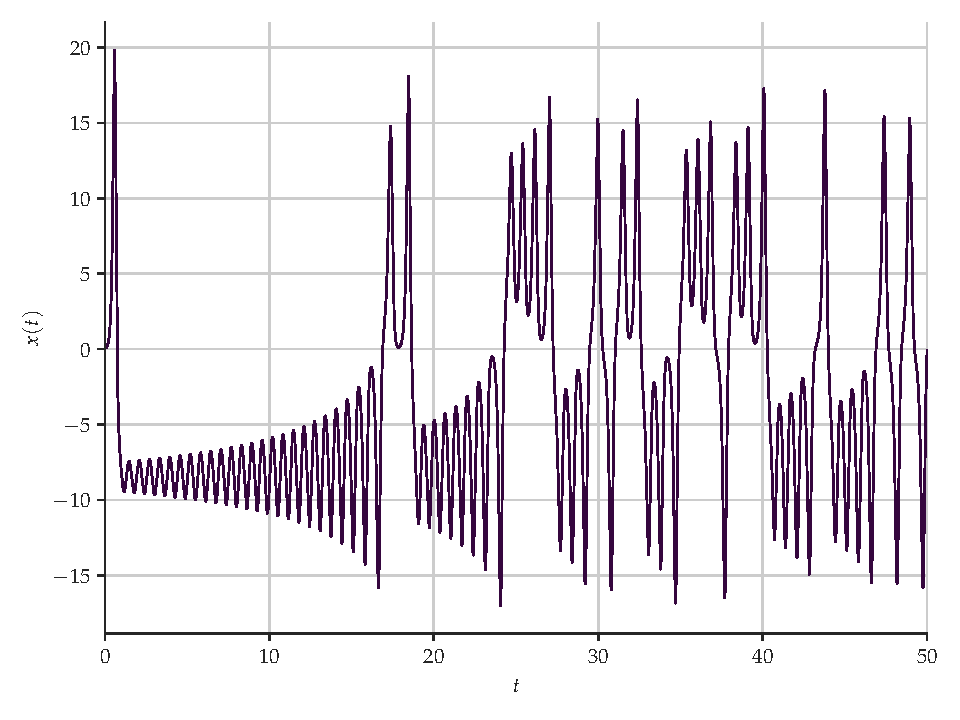
\includegraphics[scale=0.35]{serie-lorenz-x.pdf}
     \end{subfigure}
     \centering
     \begin{subfigure}[t]{0.35\textwidth}
         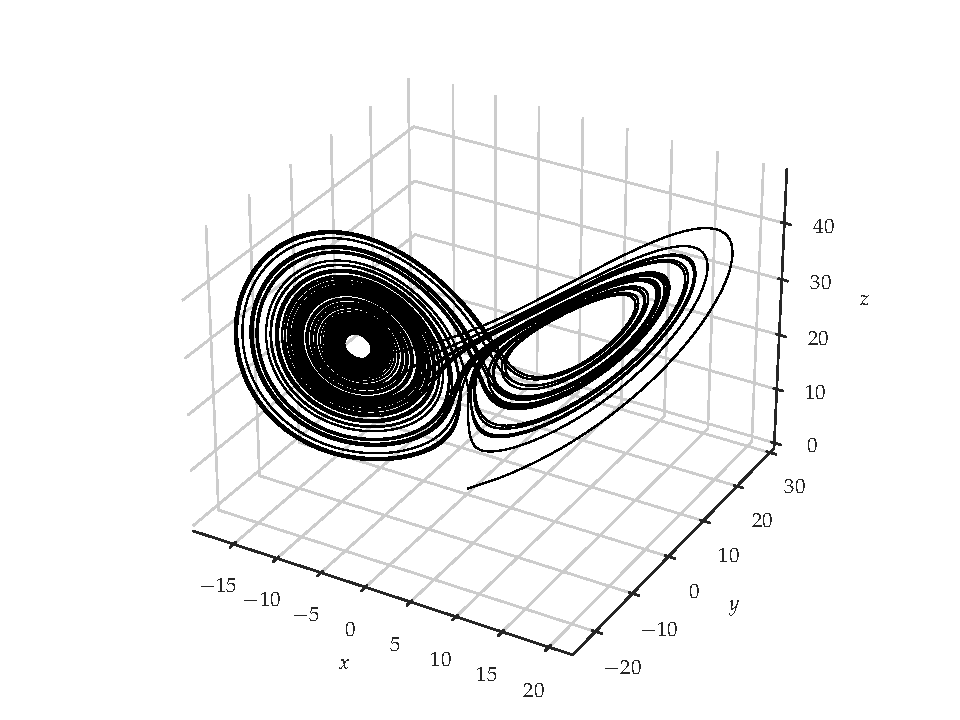
\includegraphics[scale=0.39]{diagrama-de-fases-lorenz.pdf}
     \end{subfigure}
     \caption{À esquerda, a série temporal em $x$ do sistema de Lorenz simulado e, à direita, o diagrama de fases correspondente à simulação.}
     \label{fig:lorenz}
\end{figure}


\subsection{Mapa de Hénon}

O mapa de Hénon foi um dos sistemas a tempo discreto escolhidos para esta pesquisa. Esse sistema foi proposto pelo astrônomo e matemático francês  Michel Hénon em 1976 como um modelo simplificado de uma seção de Poincaré do atrator de Lorenz, sendo descrito pelas equações abaixo \cite{henon1976two}:
\begin{subequations}
\begin{equation}
x[n+1] = y[n] + 1 - a\cdot (x[n])^2
\end{equation}
\begin{equation}
y[n+1] = b \cdot x[n]
\end{equation}
\end{subequations}
onde $a$ e $b$ são valores reais.

A presença de dinâmica caótica neste sistema discreto irá depender dos valores dos parâmetros $a$ e $b$. Hénon mostrou em sua pesquisa que, para $a = 1.4$ e $b = 0.3$, há a presença de um atrator estranho no diagrama de fases desse sistema dinâmico discreto. 

Vale mencionar que o mapa de Hénon realiza um mapeamento de dois pontos, chamados de pontos fixos. Para os valores dos parâmetros $a$ e $b$ mencionados anteriormente, tais pontos são dados por:
$$x = \frac{\sqrt{609}-7}{28} \approx 0.631354477$$
$$y = \frac{3(\sqrt{609}-7)}{280} \approx 0.189406343$$

Um desses pontos está sobre o atrator e é instável. Tal instabilidade é confirmada quando é realizada uma análise da trajetória com outros pontos próximos a este, onde percebe-se que, dependendo da região do atrator pela qual o ponto em análise se aproxima do ponto fixo, a trajetória irá divergir ou convergir para o ponto no atrator. 

A figura \ref{fig:henon} mostra a série temporal referente à variável $x$ e o atrator obtido com a simulação para $[x[0]\; y[0]]^T = [1\; 0]^T$.
\begin{figure}[H]
     \begin{subfigure}[t]{0.35\textwidth}
         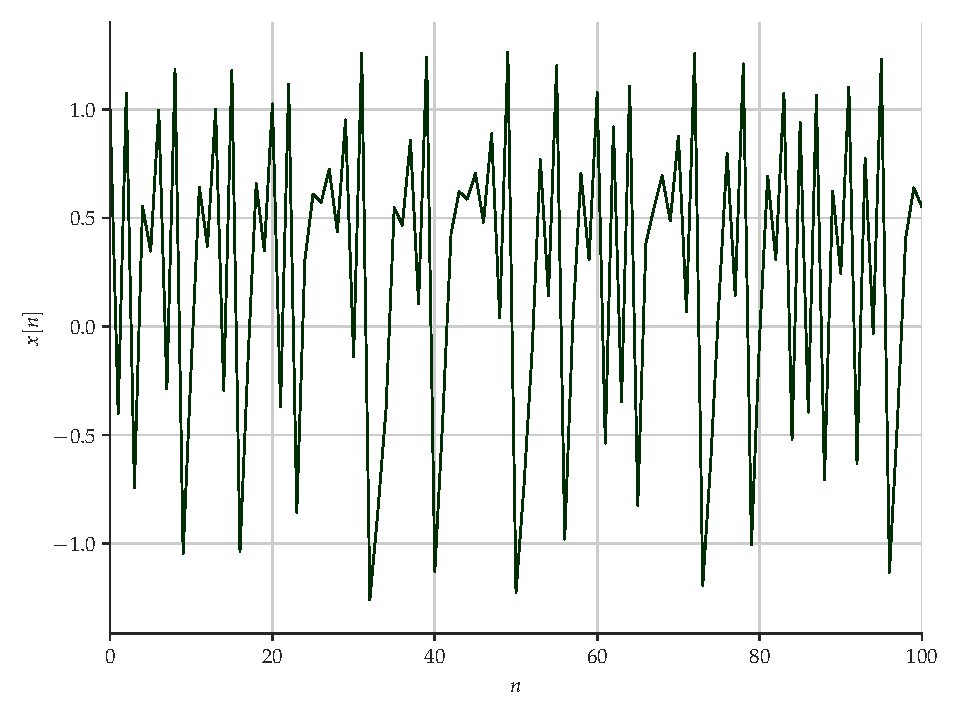
\includegraphics[scale=0.35]{serie-henon-x.pdf}
         %\caption{$y=5/x$}
     \end{subfigure}
     \centering
     \begin{subfigure}[t]{0.35\textwidth}
         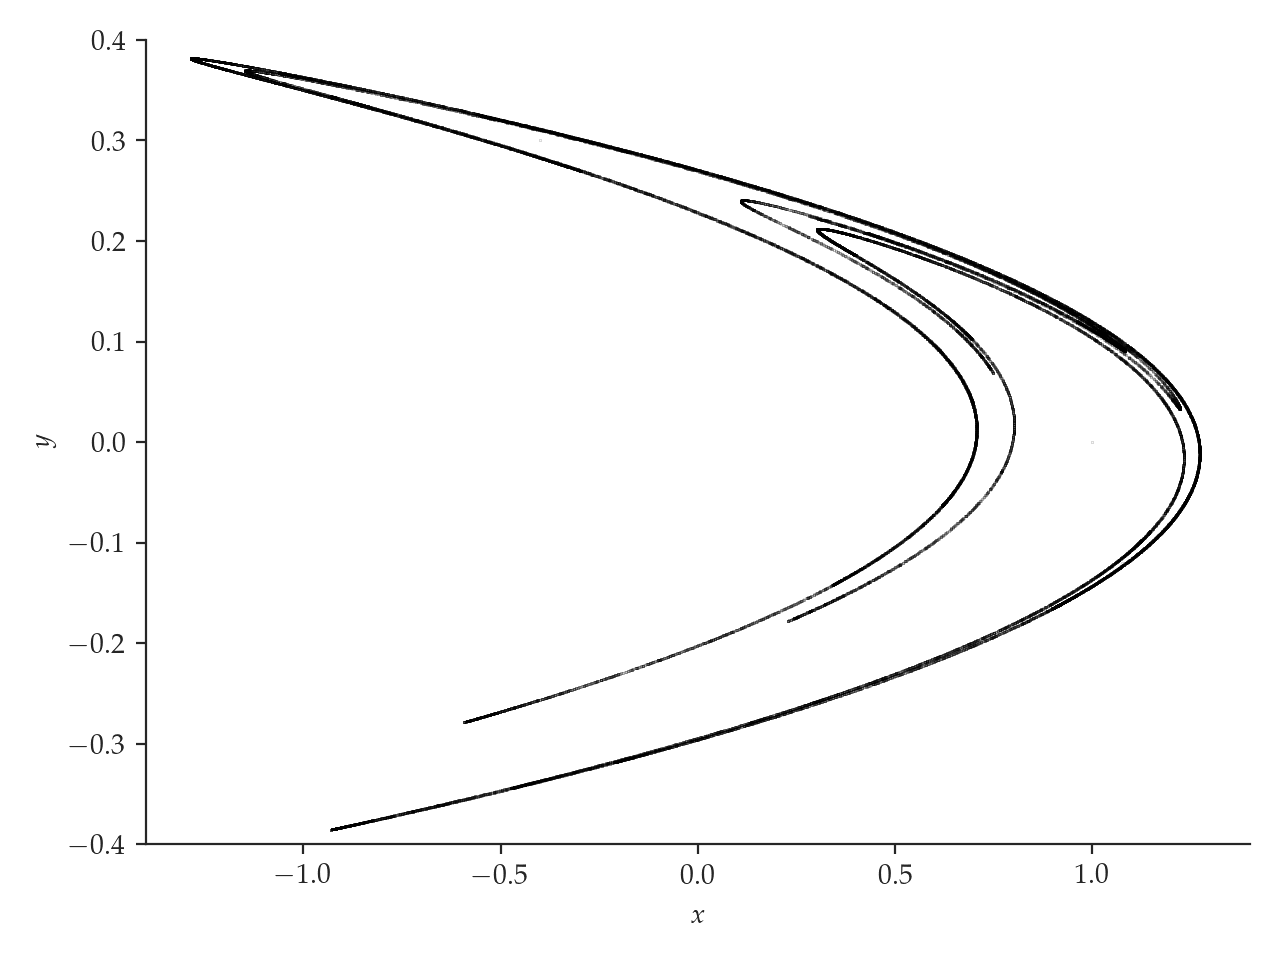
\includegraphics[scale=0.35]{mapa-de-henon.png}
         %\caption{$y=x$}
     \end{subfigure}
     \caption{À esquerda, as cem primeiras iterações da série temporal em $x$ do mapa de Hénon e, à direita, o atrator correspondente à simulação.}
     \label{fig:henon}
\end{figure}

\subsection{Mapa logístico}

Descrito em 1976 pelo biólogo e matemático Robert May, o mapa logístico representa uma das formas de modelar a população de uma determinada espécie em certos instantes de tempo \cite{may1976simple}. A equação a diferenças que descreve esse sistema pode ser vista abaixo:
\begin{equation}\label{eq:logistic}
x[n+1] = r\cdot x[n] \cdot (1 - x[n])
\end{equation}
sendo $x[n]$ um número real entre $0$ e $1$ que representa a razão entre o tamanho atual da população e o tamanho máximo desta, enquanto $r$ é um valor real entre $0$ e $4$ que representa a taxa de crescimento desta população. 

Dependendo do valor de $r$, o sistema descrito em (\ref{eq:logistic}) pode ou não operar em caos. Robert May, através de análises numéricas \cite{gleick1998chaos}, viu que para valores maiores que $3.44949$, o sistema entra em regime caótico. Interessantemente, ao aumentar mais o valor do parâmetro $r$, o cientista percebeu que há certas zonas de estabilidade, onde o sistema volta a convergir para um ciclo-limite. 

Inicialmente, após sair do regime caótico, a dinâmica terá período $2$, e, com o aumento de $r$, o sistema começa a ter período $4$, $8$, $16$, $32$, e assim por diante, até voltar, novamente, ao cenário caótico. Esse padrão de ir do caos à estabilidade para, então, voltar ao regime caótico, se repete até que $r$ atinja seu valor máximo.

Quando o físico e matemático Mitchell Feigenbaum estudou esse fenômeno, também presente em outros sistemas caóticos e em certas estruturas fractais, percebeu que a razão entre o comprimento de dois intervalos sucessivos de bifurcação tende a $\delta \approx 4.66920$ \cite{feigenbaum1978quantitative}. Esse valor é chamado de constante de Feigenbaum, não estando relacionado a nenhuma outra propriedade matemática ou constante da natureza conhecida até então.

Como o estudo visa analisar o desempenho para sistemas caóticos, foi utilizado $r=3.86$, que, conforme será visto no diagrama de bifurcação abaixo, faz com que a série temporal dada pela equação (\ref{eq:logistic}) opere em caos. 

A figura \ref{fig:logistic} indica a série temporal obtida partindo de $x[0] = 0.5$ e o diagrama de bifurcação, onde a faixa vermelha representa $r = 3.86$, para este sistema de equações.
\begin{figure}[H]
     \begin{subfigure}[t]{0.32\textwidth} 
         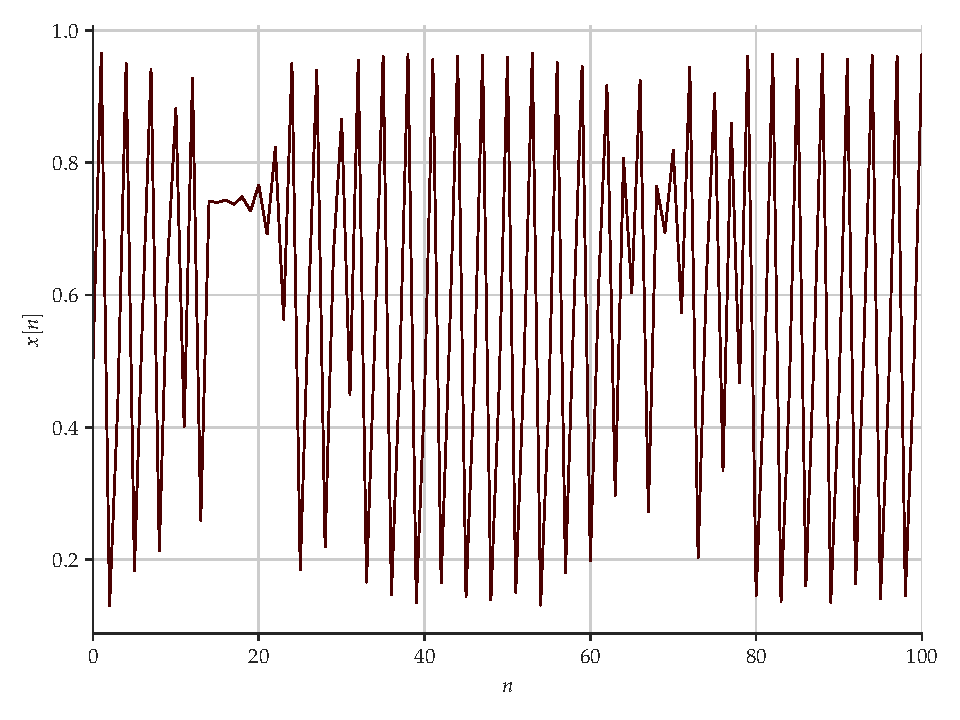
\includegraphics[scale=0.32]{serie-logistico.pdf}
         %\caption{$y=5/x$}
     \end{subfigure}
     \centering
     \begin{subfigure}[t]{0.32\textwidth} 
         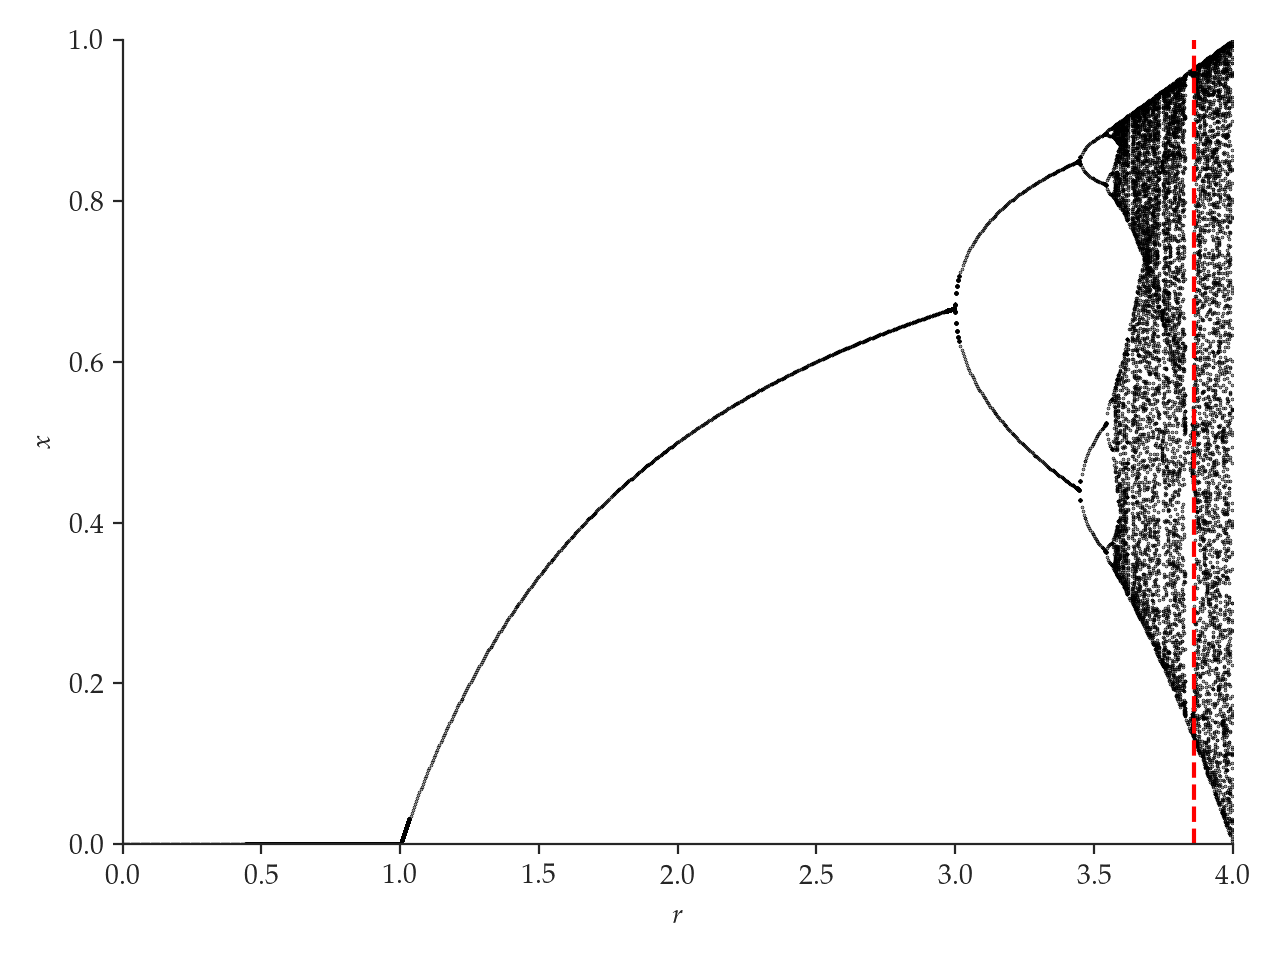
\includegraphics[scale=0.32]{mapa-logistico.png}
         %\caption{$y=x$}
     \end{subfigure}
     \centering
     \begin{subfigure}[t]{0.32\textwidth} 
         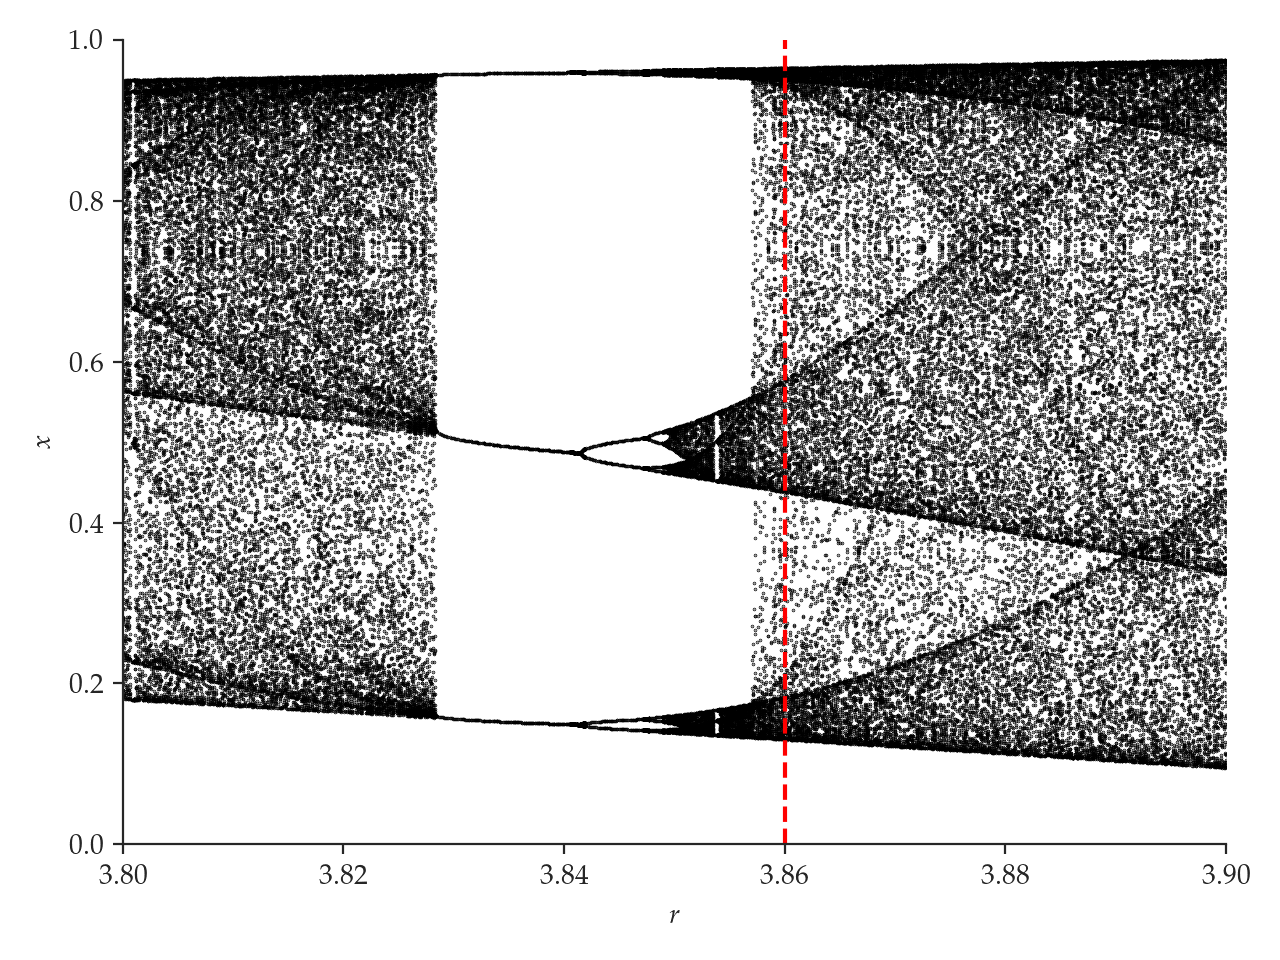
\includegraphics[scale=0.32]{mapa-logistico-zoom.png}
         %\caption{$y=x$}
     \end{subfigure}
     \caption{À esquerda, as cem primeiras iterações da série temporal do mapa logístico, ao centro, o diagrama de bifurcação deste sistema e, à direita, a seção do diagrama de bifurcação que contém o valor de $r$ utilizado.}
     \label{fig:logistic}
\end{figure}

\subsection{Equações de Mackey-Glass}

Por fim, o último sistema caótico simulado, também contínuo, está associado às equações de Mackey-Glass, as quais modelam o controle hormonal da produção de células brancas do sangue e podem ser vistas abaixo \cite{mackey1977oscillation}:
\begin{subequations}
\begin{equation}
\frac{dP(t)}{dt} = \frac{\beta_0\cdot \theta^n}{\theta^n + P(t - \tau)^n} - \gamma\cdot P(t)
\end{equation}
\begin{equation}\label{eq:mackey-glass-chaos}
\frac{dP(t)}{dt} = \frac{\beta_0\cdot \theta^n \cdot P(t - \tau)}{\theta^n + P(t - \tau)^n} - \gamma\cdot P(t)
\end{equation}
\end{subequations}
sendo $P(t)$ a densidade de tais células em um instante de tempo e $\beta_0$, $\theta$, $n$, $\tau$ e $\gamma$ valores reais relacionados a certos parâmetros hormonais de um organismo, geralmente sendo determinados experimentalmente.

Neste caso, conforme demonstrado em \cite{mackey1977oscillation}, a equação (\ref{eq:mackey-glass-chaos}) exibe comportamento caótico para valores mais altos de $\tau$. Além disso, os pesquisadores perceberam que regimes caóticos dessa equação estão correlacionados com certos problemas fisiológicos nos nossos organismos \cite{mackey1977oscillation}.

Para a simulação numérica, utilizamos $n = 10$, $\gamma = 0.1$, $\beta = 0.2$, $\theta = 1$, $\tau = 22$, $dt = 1.0$ e $P(0^-)=0.1$, gerando novamente $5000$ amostras. A série e o atrator obtidos podem ser vistos na figura \ref{fig:mackey-glass}.
\begin{figure}[!ht]
     \begin{subfigure}[t]{0.35\textwidth}
         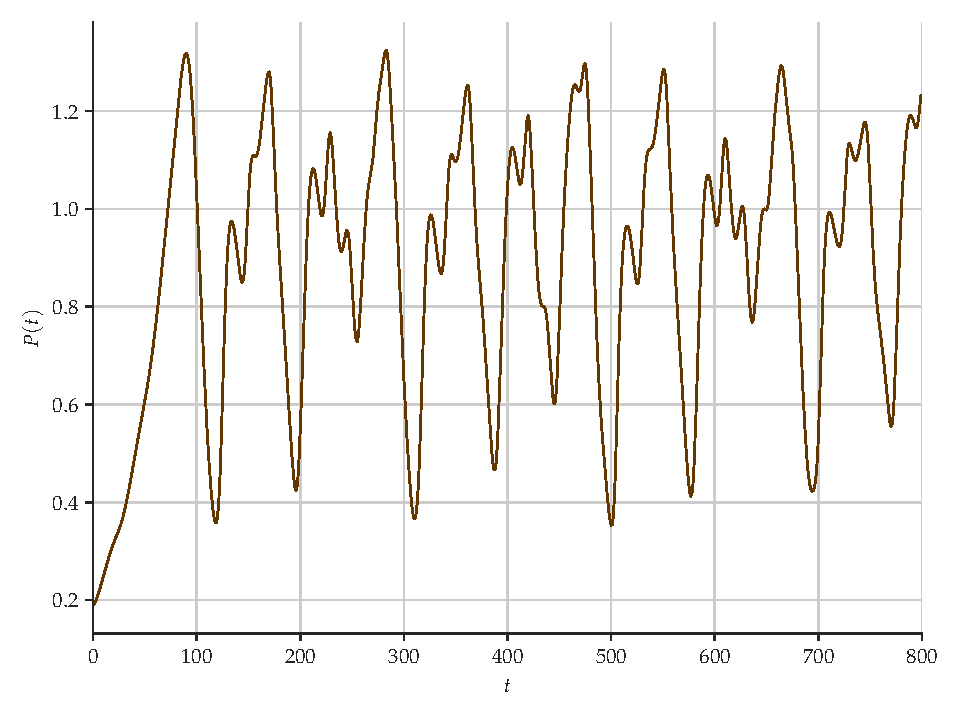
\includegraphics[scale=0.35]{serie-mackeyglass.pdf}
         %\caption{$y=5/x$}
     \end{subfigure}
     \centering
     \begin{subfigure}[t]{0.35\textwidth}
         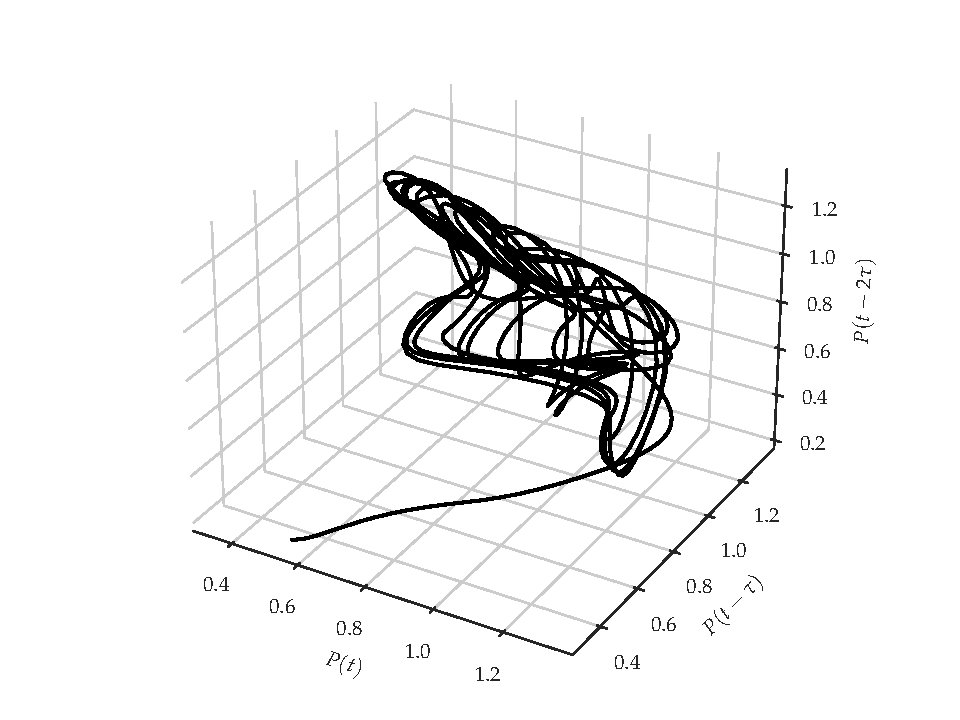
\includegraphics[scale=0.39]{atrator-mackeyglass.pdf}
         %\caption{$y=x$}
     \end{subfigure}
     \caption{À esquerda, a série temporal da equação (\ref{eq:mackey-glass-chaos}) exibida de $t = 0 $ a $t = 800$ e, à direita, o atrator correspondente à simulação.}
     \label{fig:mackey-glass}
\end{figure}

Com isso, finalizamos a exposição sobre os cenários de sistemas com dinâmica caótica escolhidos para a análise comparativa. Na próxima seção, falaremos a respeito dos dois tipos de redes neurais que incorporamos à pesquisa nesta segunda etapa. Em seguida, apresentaremos a metodologia aplicada no treinamento e análise de todos os modelos de previsão estudados, assim como as particularidades para cada caso.

\section{Modelos estudados}

Como o estudo de redes neurais artificiais foi iniciado na primeira metade da pesquisa, uma exposição mais detalhada dos fundamentos destes modelos (no caso, as redes MLP e as rede recorrentes LSTM) pode ser vista no relatório parcial.

Assim, as próximas duas subseções abordarão especificamente as redes recorrentes GRU e ESN.

\subsection{\textit{Gated Recurrent Unit} (GRU)}

Como já mencionamos anteriormente, as redes recorrentes \textit{Gated Recurrent Unit} possuem células computacionais semelhantes às células das redes LSTM, apresentadas no relatório parcial. Sua estrutura interna pode ser vista na figura \ref{fig:gru-cell}, juntamente com as equações que a descrevem.
\begin{figure}[H]
\begin{minipage}{0.4\textwidth}
\begin{center}
\scalebox{0.9}{
\begin{tikzpicture}[
    % GLOBAL CFG
    font=\sf \scriptsize,
    >=LaTeX,
    % Styles
    cell/.style={% For the main box
        rectangle, 
        rounded corners=5mm, 
        draw,
        very thick,
        },
    operator/.style={%For operators like +  and  x
        circle,
        draw,
        inner sep=-0.5pt,
        minimum height =.2cm,
        },
    function/.style={%For functions
        ellipse,
        draw,
        inner sep=1pt
        },
    ct/.style={% For external inputs and outputs
        circle,
        draw,
        line width = .75pt,
        minimum width=1cm,
        inner sep=1pt,
        },
    gt/.style={% For internal inputs
        rectangle,
        draw,
        minimum width=4mm,
        minimum height=3mm,
        inner sep=1pt
        },
    mylabel/.style={% something new that I have learned
        font=\tiny\sffamily
        },
    ArrowC1/.style={% Arrows with rounded corners
        rounded corners=.25cm,
        thick,
        },
    ArrowC2/.style={% Arrows with big rounded corners
        rounded corners=.5cm,
        thick,
        }
    ]

%Start drawing the thing...    
    % Draw the cell: 
    \node [cell, minimum height =4cm, minimum width=6cm] at (0,0){} ;

    % Draw inputs named ibox#
    \node [gt] (ibox1) at (-1.5,-0.75) {$\sigma$};
    \node [gt] (ibox2) at (0,-1.2) {$\sigma$};

   % Draw opérators   named mux# , add# and func#
    \node [operator] (mux1) at (-1.5,0) {$\times$};
    \node [operator] (mux2) at (0,1.5) {$\times$};
    \node [operator] (mux4) at (2.5,0.75) {$\times$};
    \node [operator] (add1) at (2.5,1.5) {+};    
    \node [function] (func1) at (2.5,0) {$\tanh$};
    \node [operator] (min1) at (1.25,0.75) {{\scalebox{0.5}{$-1$}}};

    % Draw External inputs? named as basis c,h,x
    \node[] (h) at (-4,1.5) {$\mathbf{h}(n-1)$};
    \node[] (x) at (0,-3) {$\mathbf{x}(n)$};

    % Draw External outputs? named as basis c2,h2,x2
    \node[] (h2) at (4,1.5) {$\mathbf{h}(n)$};
    \node[] (x2) at (2.5,3) {$\mathbf{y}(n)$};
    
    % Draw internals functions, named as basis fi,ii,ci,oi
    \node[] (ri) at (-1.85,-0.35) {$\mathbf{r}(n)$};
    \node[] (zi) at (0.4,-0.85) {$\mathbf{z}(n)$};  
    \node[] (gi) at (2.1,0.4) {$\mathbf{g}(n)$}; 
    
% Start connecting all.
    %Intersections and displacements are used. 
    % Drawing arrows    
    \draw [->, ArrowC1] (h) -- (mux2);
    \draw [->, ArrowC1] (h -| ibox1)++(-1,0) |- (ibox1);

    % Inputs

    % Internal
    \draw [->, ArrowC2] (ibox1) -- (mux1);
    
    \draw [->, ArrowC2] (ibox2) -- (mux2);
    \draw [->, ArrowC2] (mux4) -- (add1);
    \draw [->, ArrowC2] (func1) -- (mux4);
   % \draw [->, ArrowC1] (add1 -| func1)++(-0.5,0) -| (func1);

    %Outputs
    \draw [ArrowC1, ->] (mux2) -- (add1);
    \draw [ArrowC1, ->] (add1) -- (h2);
    \draw (h2 -| x2) ++(0,-0.1) coordinate (i1);
    \draw [->, ArrowC1] (h -| mux1)++(-0.5,0) |- (mux1);
    %\draw (h -- mux1) ++(-2,2) coordinate (mux1);
    \draw [->, ArrowC2] (i1)++(0,0.2) -- (x2);
    \draw [->, ArrowC1] (x -| ibox1) ++ (+1.5,+1.25) -| (ibox1);
    \draw [->, ArrowC1] (x -| func1) ++ (-2.5,+1.25) -| (func1);
    \draw [->, ArrowC1] (x) -- (ibox2);
   % \draw [->, ArrowC1] (mux1) -- (func1);
    \draw [->, ArrowC2] (mux1 -| func1)++(-2.4,0) -- (func1) coordinate (i1);
    \draw [ArrowC1] (mux1) -- ++(+1.4,0);
    \draw [->, ArrowC1] (min1) -- (mux4);
    \draw [->, ArrowC1] (ibox2) |- (min1);

\end{tikzpicture}}
\end{center}
\end{minipage}
\; \; \; \; \; \; \;
\begin{minipage}{0.4\textwidth}
\begin{center}
{ \footnotesize
$$$$
$$\mathbf{z}(n) = \sigma \left(\mathbf{W}_z [\mathbf{h}(n-1), \mathbf{x}(n)] + \mathbf{b}_z \right)$$
$$\mathbf{r}(n) = \sigma \left(\mathbf{W}_r [\mathbf{h}(n-1), \mathbf{x}(n)] + \mathbf{b}_r \right)$$
$$\mathbf{g}(n) = \tanh \left(\mathbf{W}_g [\mathbf{r}(n) \otimes \mathbf{h}(n-1), \mathbf{x}(n)]  + \mathbf{b}_g \right)$$
$$\mathbf{y}(n) = \mathbf{h}(n) = \mathbf{z}(n) \otimes \mathbf{h}(n-1) + (1 - \mathbf{z}(n)) \otimes \mathbf{g}(n)$$
}
\end{center}
\end{minipage}
\caption{Estrutura e equações de uma célula GRU.}
\label{fig:gru-cell}
\end{figure}

Ao contrário da LSTM, a célula GRU explora um único vetor de estados $\mathbf{h}(n)$. No caso, o vetor $\mathbf{z}(n)$ determina se a memória armazenada em $\mathbf{h}(n-1)$ será mantida ou apagada, enquanto o vetor $\mathbf{g}(n)$ traz a informação nova que será agregada ao vetor de estados, sendo um reflexo do estado anterior e da entrada atual ($\mathbf{x}(n)$). 

Intuitivamente, pelo fato de as GRUs serem, em essência, uma versão mais simples das redes LSTM, não seria surpreendente se as LSTM alcançassem um melhor desempenho. Entretanto, conforme verificado em \cite{cho2014learning}, a GRU pode ser superior à LSTM em determinadas aplicações. Quanto à implementação em si, existe uma grande similaridade entre GRU e LSTM (especialmente se trabalhamos com pacotes que fornecem estas camadas para uso dentro de uma arquitetura neural, como é o caso do Keras/Tensorflow). 

\subsection{\textit{Echo State Network} (ESN)}

As redes neurais com estados de eco também são modelos recorrentes para processamento da informação, à semelhança da LSTM e da GRU. No entanto, apresentam um modo de operação e um esquema de treinamento bem diferentes  \cite{boccato2013novas}. 

A figura \ref{fig:esn-model} apresenta a estrutura interna de uma rede ESN.
\begin{figure}[H]
\centering
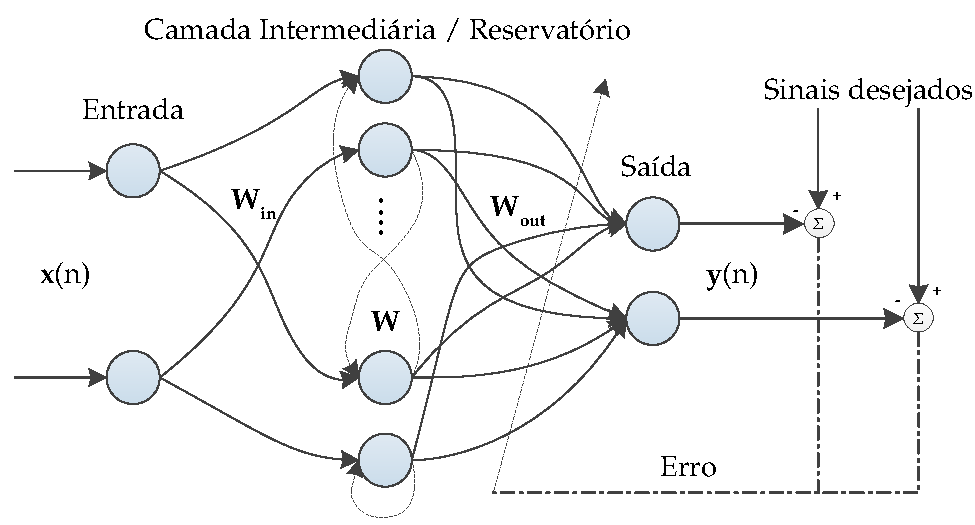
\includegraphics[scale = 0.8]{esn-network.pdf}
\caption{Estrutura típica de uma rede ESN (figura adaptada de \cite{boccato2013novas}).}
\label{fig:esn-model}
\end{figure}

As equações em (\ref{eq:esn}) descrevem a ESN, sendo $\mathbf{x}(n)$ o vetor de entrada, $\mathbf{W}_{in} \in \mathbb{R}^{N \times K}$ os pesos da camada de entrada, $\mathbf{u}(n)$ o vetor que representa as ativações dos $N$ neurônios não-lineares totalmente conectados do reservatório, representando os estados da rede, $\mathbf{W} \in \mathbb{R}^{N \times N}$ os pesos das conexões recorrentes do reservatório, $\mathbf{f}(\cdot)$ denota as funções de ativação das unidades internas da rede, $\mathbf{W}_{out} \in \mathbb{R}^{L \times N}$ é a matriz dos pesos da camada de saída e, por fim, $\mathbf{y}(n)$ denota as saídas da rede.
\begin{subequations}\label{eq:esn}
\begin{equation} \label{eq:esn-1}
\mathbf{u}(n+1) = \mathbf{f}(\mathbf{W}_{in} \cdot \mathbf{x}(n+1) + \mathbf{W} \cdot \mathbf{u}(n)) 
\end{equation}
\begin{equation} \label{eq:esn-2}
\mathbf{y}(n+1) = \mathbf{W}_{out} \cdot \mathbf{u}(n+1)
\end{equation}
\end{subequations}

O grande diferencial prático desta rede é que os pesos das conexões recorrentes dentro do reservatório $\mathbf{W}$ são ajustados com valores fixos antes do treinamento da camada de saída. Em suma, esses parâmetros são determinados tendo em vista a propriedade de estados de eco, a qual assegura que o vetor de estados da rede tende a ser guiado por um histórico recente das entradas da rede, não mais sofrendo influência dos estados iniciais, desde que condições específicas ligadas à matriz de pesos recorrentes ($\mathbf{W}$) sejam satisfeitas. Conforme demonstrado em \cite{yildiz2012re} e \cite{gallicchio2018design}, existem alguns métodos simples para a criação aleatória dos pesos que garantam a propriedade. 

A definição formal das propriedades de estado de eco é feita sob as seguintes condições \cite{boccato2013novas}:

\begin{enumerate}
\item os sinais de entrada são extraídos de um espaço compacto \footnote{ A definição de espaços compactos foi apresentada em \cite{alexandroff1929memoire}.} $\mathcal{U}$;
\item os estados da rede estão sempre contidos em um conjunto compacto $\mathcal{A} \subset \mathbb{R}^N$ de estados admissíveis, o que significa que a operação de atualização do vetor $\mathbf{u}(n)$, mostrada na equação (\ref{eq:esn-1}), sempre preserva os estados dentro de $\mathcal{A}$.
\end{enumerate}

Utilizando essas restrições, o autor da arquitetura ESN apresentou duas novas condições para a existência das propriedades de estado de eco. 

A primeira condição mostra que, caso o máximo valor singular da matriz
de pesos do reservatório $\mathbf{W}$, em módulo, esteja dentro do círculo unitário ($|\sigma_{max} (\mathbf{W})| < 1$), a rede recorrente apresenta estados de eco \cite{jaeger2001echo, jaeger2002short}.

A segunda condição estabelece a não-existência de estados de eco em função do raio espectral, i.e., do autovalor de maior módulo da matriz de pesos internos $\mathbf{W}$, denotado por $\rho_s (\mathbf{W})$: se $\rho_s (\mathbf{W}) > 1$, então a rede não possui estados de eco \cite{jaeger2001echo}. Para isto, além das restrições apresentadas anteriormente, é assumido que a entrada é nula.

Neste caso, considerando que os pesos internos da rede $\mathbf{W}$ representam uma espécie de reservatório de dinâmicas que, por sua vez, deve gerar um conjunto de comportamentos dinâmicos o mais diversificado possível, a matriz de pesos $\mathbf{W}$ deve ser criada com um certo grau de esparsidade, conforme demonstrado em \cite{jaeger2001echo}. Dessa forma, um conjunto de comportamentos dinâmicos é obtido sem um conhecimento prévio do sinal que se deseja modelar.

Por fim, vale mencionar que o ajuste dos parâmetros na camada de saída pode ser realizado com um procedimento de regressão linear (neste caso, utilizando amostras passadas do sinal a ser previsto), sem necessitar de um treinamento iterativo, como nas outras redes neurais estudadas nesta pesquisa. Esse fato economiza tempo de processamento e evita os conhecidos problemas de desvanecimento e de explosão do vetor gradiente, assim como outras instabilidades que podem ocorrer no treinamento de uma rede recorrente. 

Com isso, finalizamos o restante da exposição teórica desta pesquisa. A próxima seção descreverá  a metodologia utilizada nesta análise.

\section{Metodologia}

Nesta segunda parte da pesquisa de iniciação científica foram implementados modelos preditores com base nas quatro redes neurais artificiais estudadas (MLP, LSTM, GRU e ESN) para os quatro cenários exibidos na seção 2. 

Iniciaremos a discussão com a apresentação da busca em grade realizada para  todos os modelos, de forma a determinar os parâmetros ótimos das redes neurais em cada cenário. Em seguida, utilizando os melhores parâmetros, avaliamos a progressão do erro quadrático médio em função do número de amostras de entrada $K$ do modelo preditor. Por fim, comparamos qual foi a média e o desvio padrão do EQM com o melhor valor de $K$ de cada modelo nos quatro cenários. Em todos os experimentos, o horizonte de predição utilizado foi $L=3$. Assim, iremos predizer o valor da terceira iteração à frente do valor atual da série temporal.

Vale reforçar que, para todos os modelos e cenários, utilizamos $85\%$ das amostras das séries temporais para treinamento (ou, equivalentemente, os primeiros $4250$ valores).  Além disso, o conjunto de validação, utilizado na busca em grade para avaliar a predição de uma configuração testada, corresponde a $10\%$ dos dados de treinamento (as últimas $425$ amostras). Assim, os dados de treinamento efetivamente correspondem às primeiras $3825$ amostras, os dados de validação correspondem às $425$ amostras depois destas e, por fim, o conjunto de teste corresponde aos últimos $750$ instantes de tempo. Essa proporção entre os dados de treinamento, de teste e de validação foi mantida para todas as redes analisadas.

Em seguida, na seção 4.2, será apresentada a análise da autocorrelação parcial das séries temporais, a qual norteou a definição das faixas de valores de $K$ para cada cenário. Por fim, na seção 4.3, mostramos os testes realizados com cada valor de $K$ e com cada modelo de previsão, de forma a encontrar a melhor configuração para esse parâmetro. 

\subsection{Configurações utilizadas}

Conforme dito anteriormente, foi realizada uma busca em grade com validação cruzada para determinar as melhores configurações de cada rede neural para a predição das séries temporais em cada cenário. Para cada arquitetura, um conjunto de valores candidatos foi gerado para cada hiperparâmetro e todas as combinações possíveis foram avaliadas tendo em vista o desempenho do modelo em dados de validação.

Houve algumas diferenças entre o processo realizado para a rede MLP e para as redes recorrentes tendo em vista o caráter destes modelos. Como a relação temporal entre as amostras não é importante para a MLP, a busca em grade considerou uma validação cruzada com $4$ \textit{folds} nos dados de treinamento. Ou seja, para cada configuração, foi avaliado o desempenho desta rede na predição de quatro subconjuntos das quatro séries temporais escolhidas.

Já nas redes recorrentes, foi considerado um esquema de validação do tipo \textit{holdout}. Esse processo dividiu o conjunto de treinamento (novamente composto por $85\%$ dos dados gerados) em $4$ seções. Cada seção era composta por uma fração dos dados de treinamento, sendo que cada seção incluía a seção anterior no seu conjunto de dados. Por exemplo, a segunda seção obtida pelo \textit{holdout} inclui a primeira seção e mais algumas amostras, além de uma subdivisão de validação que será utilizada para avaliar o resultado. Com isso, obtém-se conjuntos sequenciais de dados para avaliação do desempenho. Esse procedimento é necessário para as redes recorrentes, pois a relação temporal entre os dados de entrada deve ser levada em conta.

Por fim, durante esta etapa de busca dos hiperparâmetros, consideramos que  $K = 4$. 

Com esses detalhes expostos, iniciaremos a exposição com a busca em grade realizada na rede MLP para, em seguida, falarmos sobre as configurações obtidas para as redes recorrentes.

\subsubsection{MLP}

Na busca em grade para a MLP, avaliamos diferentes tamanhos de \textit{batch} ($2$, $4$, $8$, $16$, $32$), se haveria ou não uma camada de \textit{batch normalization} na entrada da rede MLP, diferentes opções de função de ativação dos neurônios na camada intermediária ($\selu$, $\relu$, $\elu$, $\tanh$, $\sigmoid$), esquemas alternativos para a inicialização dos pesos ($\glorot$, $\he$, $\lecun$, tanto com distribuição normal, quanto uniforme), diferentes quantidades de neurônios na camada intermediária ($5$, $10$, $15$, $20$, $30$, $50$, $75$, $100$) e, também, diferentes valores para a taxa de aprendizagem ($0.001$, $0.003$, $0.005$, $0.008$, $0.01$). Em todos os testes, consideramos uma rede MLP com uma única camada intermediária. 

Ao final do processo completo de busca, foram identificadas as configurações "ótimas" da rede MLP em cada cenário, as quais são exibidas na tabela  \ref{tab:mlp}.
\begin{table}[H]
\begin{center}
\scalebox{0.75}{
\begin{tabular}{c c c c c c c}
\toprule
\addlinespace
  \textbf{Cenário} & \pbox{3cm}{\centering \textbf{\textit{Batch normalization}}} & \pbox{2cm}{\centering \textbf{Tamanho do \textit{batch}}} & {\centering \textbf{Ativação}} & {\centering \textbf{Inicialização}} & \pbox{2cm}{\centering \textbf{Nº de neurônios}} & \pbox{4cm}{\centering \textbf{Taxa de aprendizagem}}\\
 \addlinespace 
 \midrule
 \addlinespace
 \pbox{2cm}{\centering \textbf{Mapa de Hénon}} & Não & $8$ & $\sigmoid$ & $\glorot\, \normal$ & $50$ & $0.003$\\  
  \addlinespace
  \hline
  \addlinespace
\pbox{2cm}{\centering \textbf{Mapa logístico}} & Não & $2$ & $\tanh$ & $\glorot\, \uniform$ & $10$ & $0.003$\\ 
  \addlinespace
  \hline
  \addlinespace
 \pbox{2cm}{\centering \textbf{Sistema de Lorenz}} & Não & $2$ & $\selu$ & $\lecun\, \normal$ & $50$ & $0.001$\\ 
  \addlinespace
  \hline
  \addlinespace
 \pbox{2.5cm}{\centering \textbf{Equações de Mackey-Glass}} & Não & $4$ & $\tanh$ & $\glorot\, \normal$ & $5$ & $0.001$\\ 
 \addlinespace
\bottomrule 
 \end{tabular}}
\caption{Melhores parâmetros para a rede MLP nos cenários em análise.}
\label{tab:mlp}
\end{center}
\end{table}

\subsubsection{LSTM e GRU}

Para as redes recorrentes LSTM e GRU, foi avaliado o tamanho do \textit{batch} ($2$, $4$, $8$, $16$, $32$), a inicialização dos pesos ($\glorot \, \uniform$, $\glorot \, \normal$), o número de neurônios recorrentes na camada intermediária ($5$, $10$, $15$, $20$, $30$, $50$, $75$, $100$), e a taxa de aprendizagem ($0.001$, $0.003$, $0.005$, $0.008$, $0.01$), novamente utilizando apenas uma camada intermediária e mantendo a função de ativação usual da célula recorrente ($\tanh$). Por conta disso, para o sistema de Lorenz, foi feito um ajuste de escala para evitar a saturação dos neurônios.

As tabelas \ref{tab:lstm} e \ref{tab:gru} exibem as melhores configurações obtidas em cada cenário para as redes LSTM e GRU, respectivamente.
\begin{table}[H]
\begin{center}
\scalebox{0.75}{
\begin{tabular}{c c c c c}
\toprule
\addlinespace
  \textbf{Cenário} & \pbox{2cm}{\centering \textbf{Tamanho do \textit{batch}}} & {\centering \textbf{Inicialização}} & \pbox{2cm}{\centering \textbf{Nº de neurônios}} & \pbox{4cm}{\centering \textbf{Taxa de aprendizagem}}\\
 \addlinespace 
 \midrule
 \addlinespace
 \pbox{2cm}{\centering \textbf{Mapa de Hénon}} & $4$ & $\glorot\, \normal$ & $15$ & $0.005$\\  
  \addlinespace
  \hline
  \addlinespace
\pbox{2cm}{\centering \textbf{Mapa logístico}} & $2$ & $\glorot\, \uniform$ & $100$ & $0.008$\\ 
  \addlinespace
  \hline
  \addlinespace
 \pbox{2cm}{\centering \textbf{Sistema de Lorenz}} & $4$ & $\glorot\, \uniform$ & $15$ & $0.003$\\  
  \addlinespace
  \hline
  \addlinespace
 \pbox{2.5cm}{\centering \textbf{Equações de Mackey-Glass}} & $2$ & $\glorot\, \uniform$ & $50$ & $0.003$\\ 
 \addlinespace
 \bottomrule
\end{tabular}}
\caption{Melhores parâmetros para a rede LSTM nos cenários em análise.}
\label{tab:lstm}
\end{center}
\end{table}

\begin{table}[H]
\begin{center}
\scalebox{0.75}{
\begin{tabular}{c c c c c}
\toprule
\addlinespace
  \textbf{Cenário} & \pbox{2cm}{\centering \textbf{Tamanho do \textit{batch}}} & {\centering \textbf{Inicialização}} & \pbox{2cm}{\centering \textbf{Nº de neurônios}} & \pbox{4cm}{\centering \textbf{Taxa de aprendizagem}}\\
 \addlinespace 
 \midrule
 \addlinespace
 \pbox{2cm}{\centering \textbf{Mapa de Hénon}} & $4$ & $\glorot\, \normal$ & $30$ & $0.003$\\    
  \addlinespace
  \hline
  \addlinespace
\pbox{2cm}{\centering \textbf{Mapa logístico}} & $2$ & $\glorot\, \normal$ & $100$ & $0.003$\\  
  \addlinespace
  \hline
  \addlinespace
 \pbox{2cm}{\centering \textbf{Sistema de Lorenz}} & $8$ & $\glorot\, \uniform$ & $30$ & $0.001$\\ 
  \addlinespace
  \hline
  \addlinespace
 \pbox{2.5cm}{\centering \textbf{Equações de Mackey-Glass}} & $2$ & $\glorot\, \uniform$ & $10$ & $0.005$\\ 
 \addlinespace
 \bottomrule
\end{tabular}}
\caption{Melhores parâmetros para a rede GRU nos cenários em análise.}
\label{tab:gru}
\end{center}
\end{table}

\subsubsection{ESN}

Para esta rede foi realizada uma busca em grade para determinar o número de neurônios no reservatório ($30$, $50$, $70$, $90$, $100$, $120$, $140$, $160$, $180$, $200$, $240$, $280$, $320$, $360$, $400$, $440$, $480$, $500$) e o valor do raio espectral ($0.1$, $0.2$, $0.3$, $0.4$, $0.5$, $0.6$, $0.7$, $0.8$, $0.9$, $0.95$, $0.96$, $0.97$, $0.98$, $0.99$), que determina o maior autovalor da matriz de pesos do reservatório. Por tratar-se de uma rede recorrente, também foi utilizado o processo de \textit{holdout} descrito na seção 4.1. Vale também mencionar que a taxa de vazamento, que representa a velocidade com a qual o reservatório atualiza suas dinâmicas, foi fixada em $0.9$ para todos os cenários.

A tabela \ref{tab:esn} exibe as melhores configurações para a ESN em cada um dos cenários. Um ponto interessante a destacar é que os melhores valores do raio espectral são relativamente pequenos e estão bem afastados de $1.0$, o que significa que o reservatório tende a desenvolver uma memória mais curta e, assim, esquecer mais rapidamente o passado. Tal característica parece fazer sentido considerando o caráter caótico das séries temporais exploradas no trabalho. 
\begin{table}[H]
\begin{center}
\scalebox{0.75}{
\begin{tabular}{c c c c c}
\toprule
\addlinespace
  \textbf{Parâmetro} & \pbox{2cm}{\centering \textbf{Mapa de Hénon}} & \pbox{2cm}{\centering \textbf{Mapa logístico}} & \pbox{2cm}{\centering \textbf{Sistema de Lorenz}} & \pbox{3.5cm}{\centering \textbf{Equações de Mackey-Glass}}\\
   \addlinespace
 \midrule
 \addlinespace
 {\centering \textbf{Nº de neurônios}} & $500$ & $500$ & $120$ & $500$\\
  \addlinespace
  \hline
  \addlinespace
 {\centering \textbf{Raio espectral}} & $0.1$ & $0.1$ & $0.2$ & $0.4$\\
 \bottomrule  
\end{tabular}}
\caption{Melhores parâmetros para a rede ESN nos cenários em análise.}
\label{tab:esn}
\end{center}
\end{table}

Com isso, concluímos a apresentação das melhores configurações para as redes neurais avaliadas em todos os cenários escolhidos. Na próxima seção, falaremos sobre outra análise realizada, dessa vez não sobre os modelos em teste, mas sim sobre certas características das séries temporais utilizadas. 

\subsection{Estudo da autocorrelação parcial das séries temporais}

Com as melhores configurações para cada rede e cenário obtidas, foi analisada a progressão do erro quadrático médio para cada valor de $K$. A faixa de valores para $K$ a ser testada foi determinada utilizando a autocorrelação parcial das séries temporais de cada sistema analisado, levando em considerações os atrasos (ou afastamentos temporais entre amostras) que apresentam correlações mais significativas. 

A figura \ref{fig:autocorrelation} mostra a autocorrelação parcial para as séries temporais utilizadas. É interessante perceber a rápida diminuição da correlação conforme o atraso entre amostras aumenta, especialmente nos casos dos sistemas discretos. 
\begin{figure}[H]
     \begin{subfigure}[t]{0.325\textwidth}
         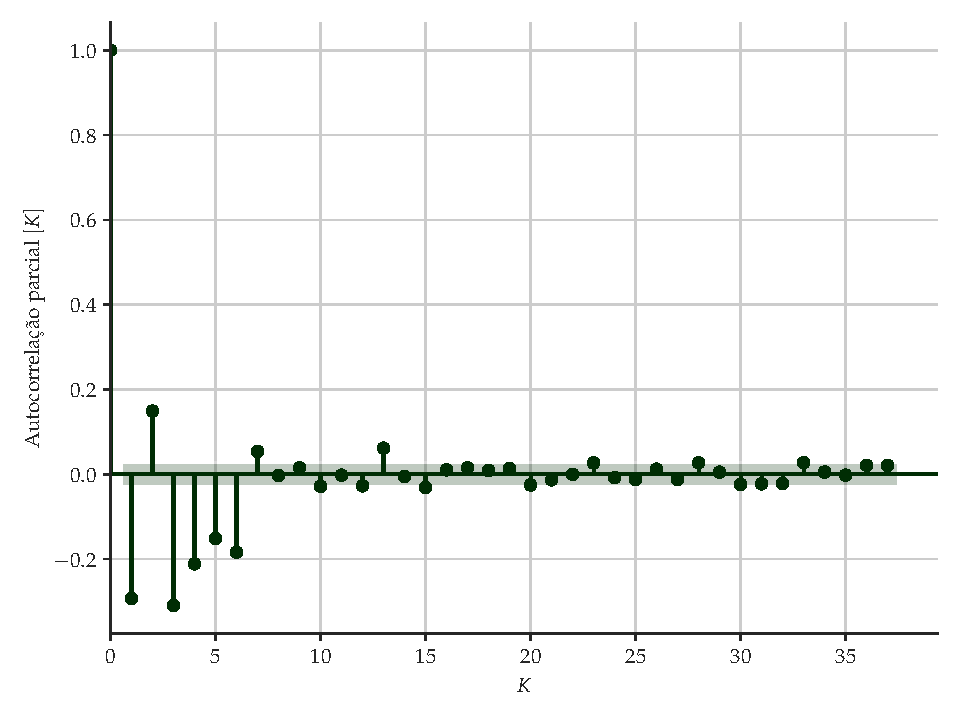
\includegraphics[scale=0.30]{autocorrelacao-parcial-henon.pdf}
         \caption{Mapa de Hénon}
     \end{subfigure}
     \centering
     \begin{subfigure}[t]{0.325\textwidth} 
         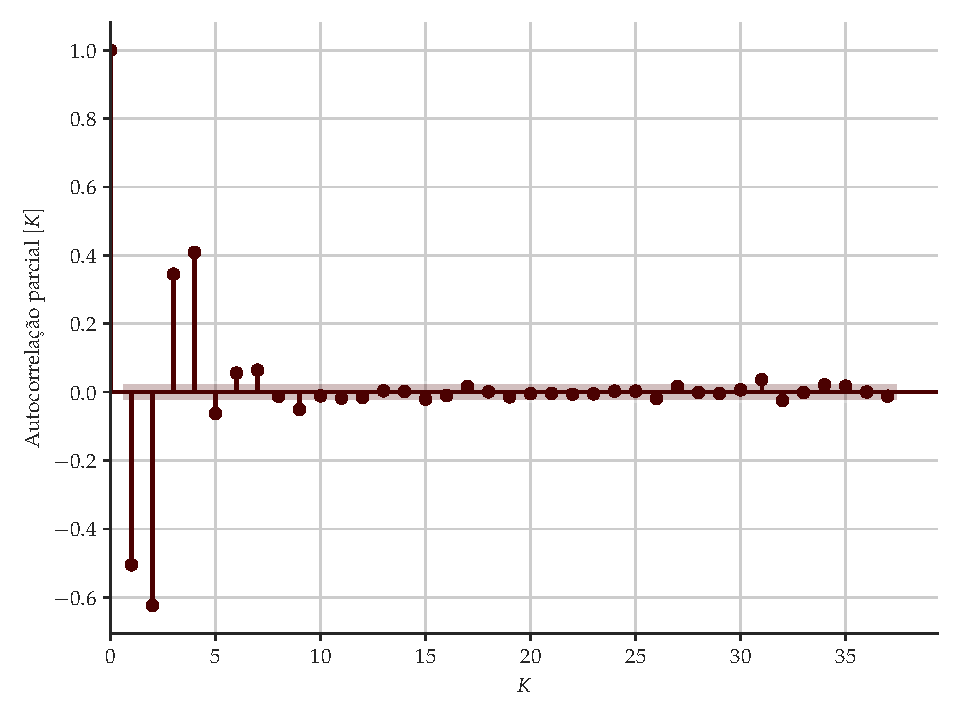
\includegraphics[scale=0.30]{autocorrelacao-parcial-logistic.pdf}
         \caption{Mapa logístico}
     \end{subfigure}
     \centering
     \\
     \begin{subfigure}[t]{0.325\textwidth}
         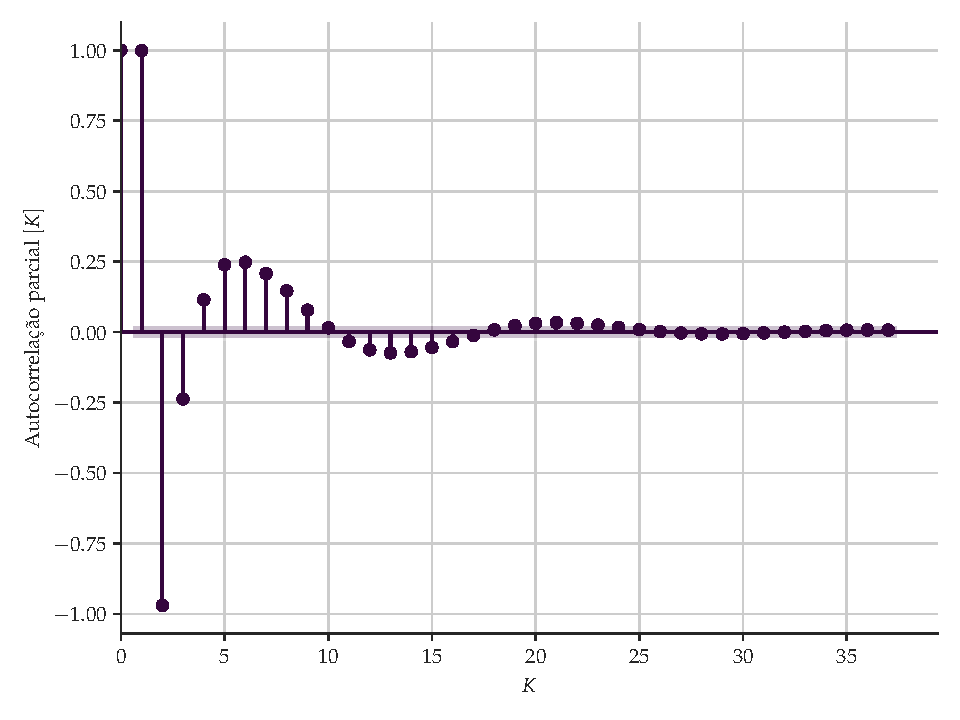
\includegraphics[scale=0.30]{autocorrelacao-parcial-lorenz.pdf}
         \caption{Sistema de Lorenz}
     \end{subfigure}
     \centering
     \begin{subfigure}[t]{0.325\textwidth} 
         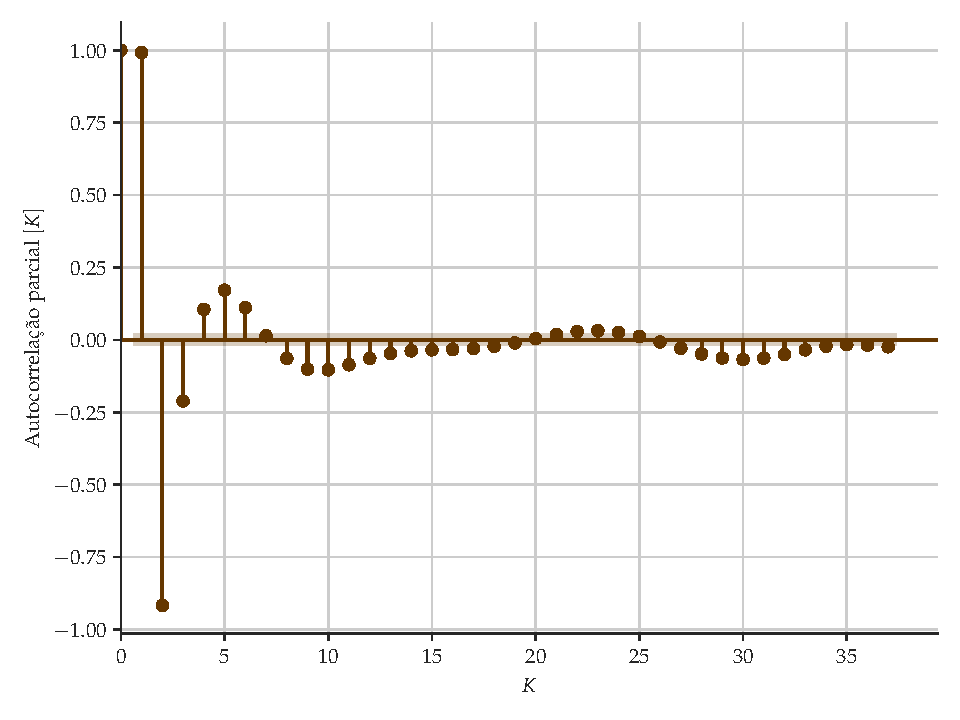
\includegraphics[scale=0.30]{autocorrelacao-parcial-mackeyglass.pdf}
         \caption{Equações de Mackey-Glass}
     \end{subfigure}  
     \centering   
     \caption{Autocorrelação parcial para as séries temporais utilizadas.}
     \label{fig:autocorrelation}
\end{figure}

Vale mencionar que a autocorrelação parcial encontra a correlação dos resíduos (assim denominados porque são obtidos após a remoção dos efeitos já explicados pelos primeiros atrasos) com o próximo valor de atraso, removendo correlações entre este e atrasos passados. Logo, essa medida descreve somente a relação direta entre duas observações da série afastadas por $K$ instantes de tempo.

A tabela \ref{tab:autocorrelation} mostra a faixa de valores para $K$ a ser testada obtida com a análise descrita nos parágrafos anteriores.
\begin{table}[H]
\begin{center}
\scalebox{0.75}{
\begin{tabular}{c c c c c}
\toprule
\addlinespace
   & \pbox{2cm}{\centering \textbf{Mapa de Hénon}} & \pbox{2cm}{\centering \textbf{Mapa logístico}} & \pbox{2cm}{\centering \textbf{Sistema de Lorenz}} & \pbox{3.5cm}{\centering \textbf{Equações de Mackey-Glass}}\\
   \addlinespace
 \midrule
 \addlinespace
 {\centering \textbf{Faixa de valores}} & $1 \thicksim 9$ & $1 \thicksim 8$ & $1 \thicksim 10$ & $1 \thicksim 7$\\
 \bottomrule
\end{tabular}}
\caption{Faixa de valores inteiros para $K$ a ser testada em cada cenário para todas as redes.}
\label{tab:autocorrelation}
\end{center}
\end{table}

\subsection{Análise do melhor valor para $K$}

Com as faixas de valores de $K$ estabelecidas, avaliamos a progressão do erro quadrático médio para diferentes configurações desse parâmetro.

Para realizar esse procedimento, cada rede (com as configurações ótimas) foi treinada utilizando $85\%$ dos dados gerados, sendo que $10\%$ dos dados de treinamento foram utilizados como o conjunto de validação (nas redes MLP, LSTM e GRU). Em seguida, com o modelo treinado, foi avaliado o EQM no conjunto de teste (que corresponde às últimas 750 amostras). Esse processo foi realizado $5$ vezes para cada $K$, obtendo assim um valor médio e desvio-padrão para cada modelo e em cada cenário. 

Além disso, como o ajuste de parâmetros da ESN possui solução em forma fechada, não foi necessário utilizar um conjunto de validação no treinamento. No caso da MLP, LSTM e GRU, o processo iterativo de ajuste dos pesos utilizou um conjunto de validação de forma a seguir o procedimento de \textit{early stopping} para evitar o sobreajuste da rede.

A figura \ref{fig:mse-progression} mostra a progressão do EQM observada em cada cenário para cada uma das redes estudadas. 
\begin{figure}[!ht]
     \begin{subfigure}[t]{0.45\textwidth} 
         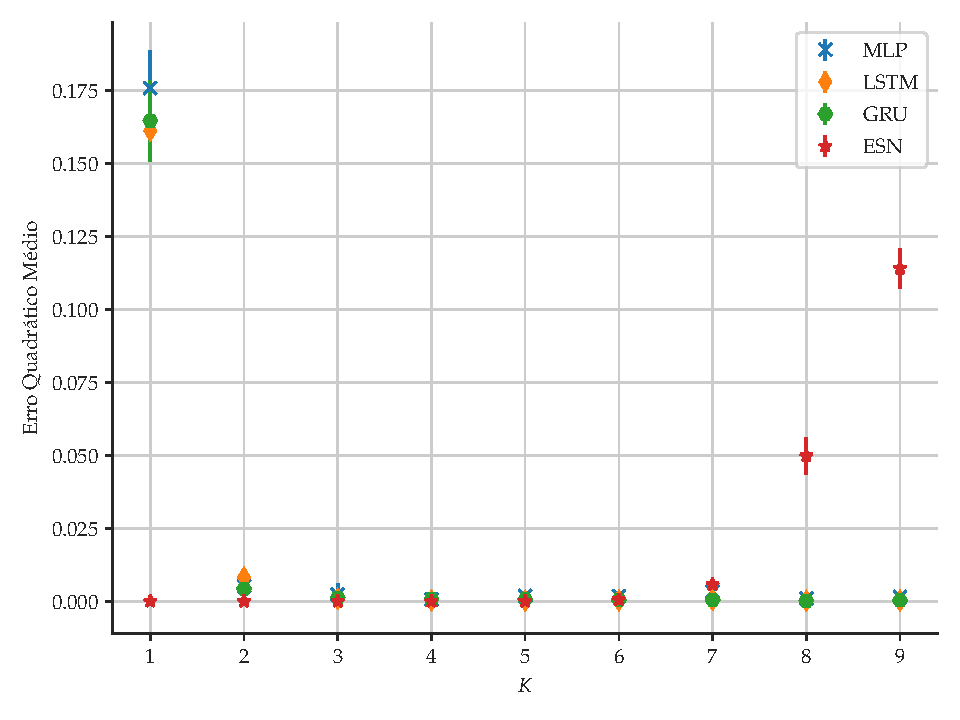
\includegraphics[scale=0.4]{progressao-k-henon.pdf}
         \caption{Mapa de Hénon}
     \end{subfigure}
     \centering
     \begin{subfigure}[t]{0.45\textwidth} 
         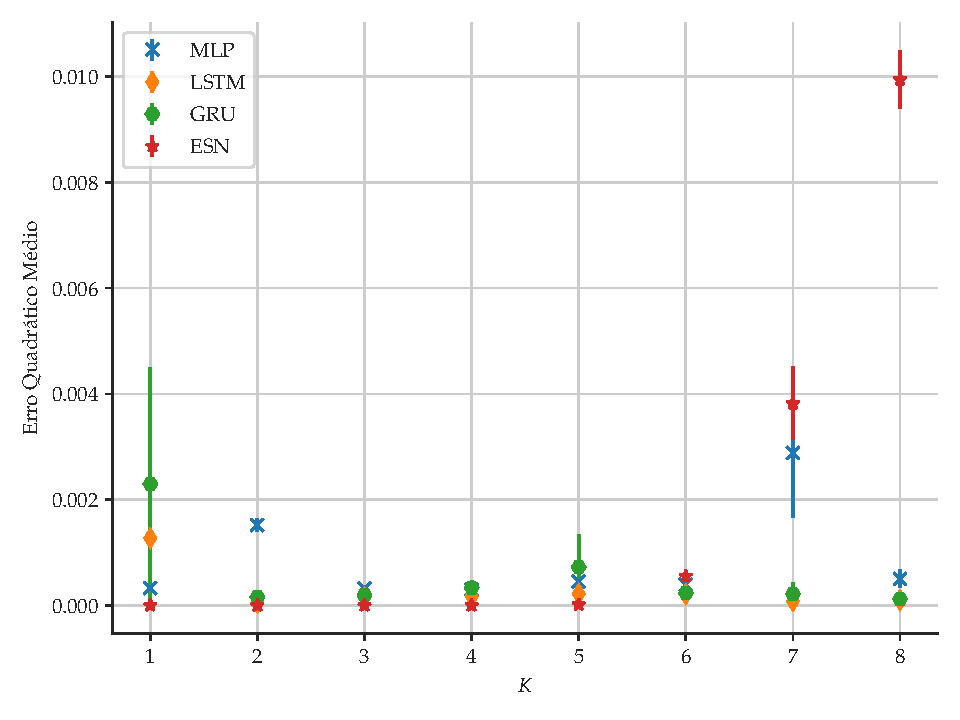
\includegraphics[scale=0.4]{progressao-k-logistic.pdf}
         \caption{Mapa logístico}
     \end{subfigure}
     \\
     \centering
     \begin{subfigure}[t]{0.45\textwidth}
         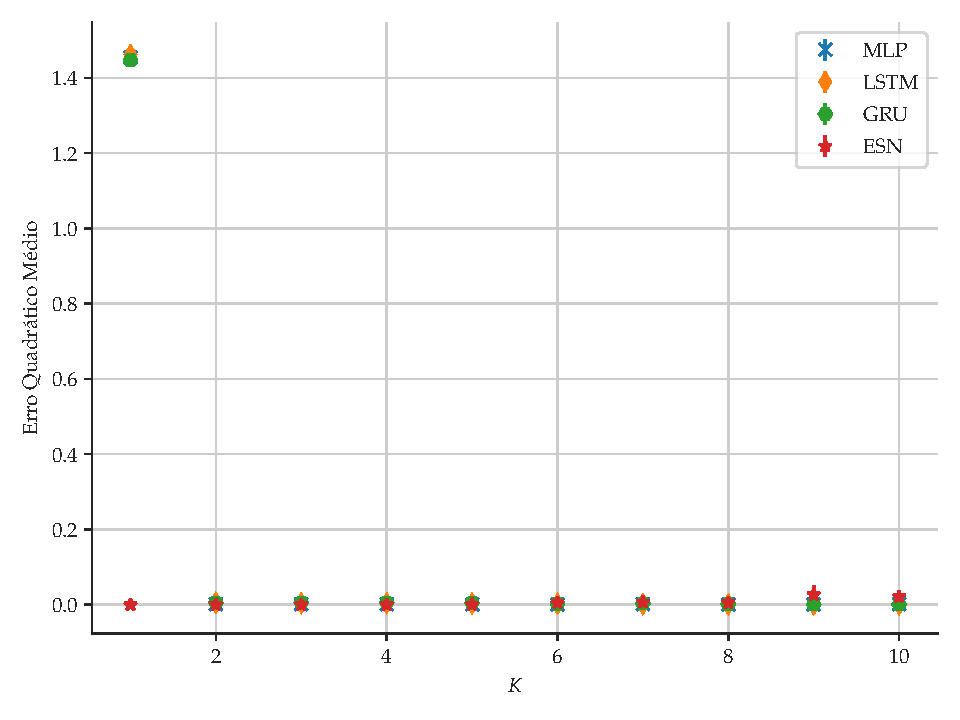
\includegraphics[scale=0.4]{progressao-k-lorenz.pdf}
         \caption{Sistema de Lorenz}
     \end{subfigure}
     \centering
     \begin{subfigure}[t]{0.45\textwidth} 
         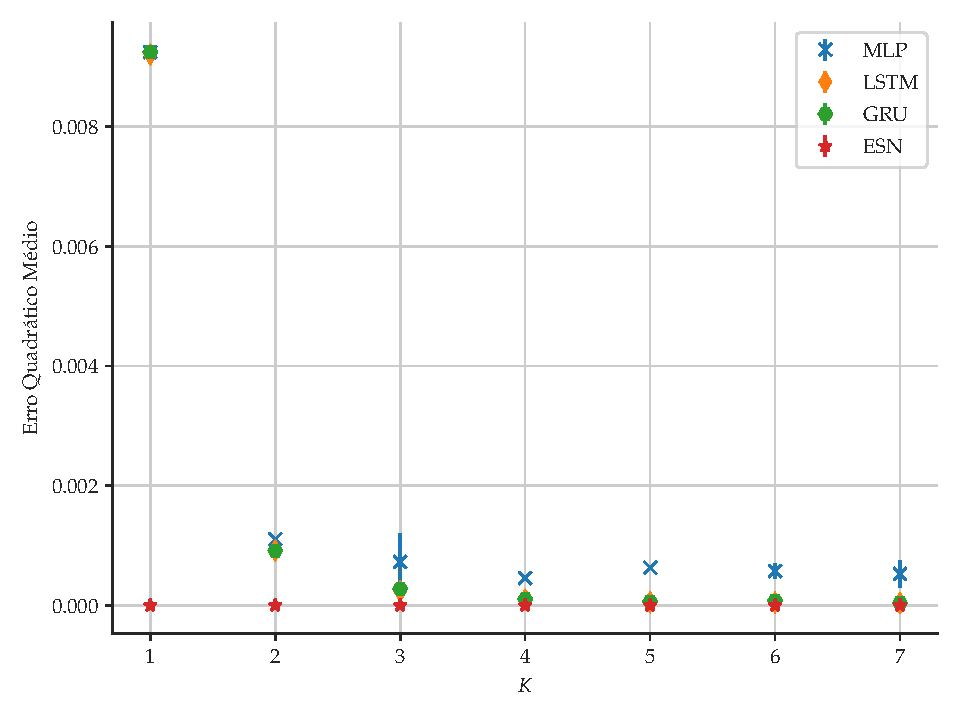
\includegraphics[scale=0.4]{progressao-k-mackeyglass.pdf}
         \caption{Equações de Mackey-Glass}
     \end{subfigure}  
     \centering   
     \caption{Progressão do erro quadrático médio para cada valor de $K$ nos cenários avaliados para todas as redes neurais testadas.}
     \label{fig:mse-progression}
\end{figure}

Nas tabelas \ref{tab:henon-eqm}, \ref{tab:logistic-eqm}, \ref{tab:lorenz-eqm} e \ref{tab:mackeyglass-eqm}, constam os valores médios e desvios-padrão referentes ao EQM para cada valor $K$ dos modelos avaliados, no cenário do mapa de Hénon, do mapa logístico, do sistema de Lorenz, e das equações de Mackey-Glass, respectivamente.
\begin{table}[H]
\begin{center}
\begin{subtable}{1\textwidth}
\begin{center}
\scalebox{0.47}{
\begin{tabular}{c c c c c}
\toprule
\addlinespace
 $\bm{K}$ & {\centering \textbf{MLP}} & {\centering \textbf{LSTM}} & {\centering \textbf{GRU}} &  {\centering \textbf{ESN}} \\
   \addlinespace
 \midrule
 \addlinespace
 $\bm{1}$ & $(1.758 \pm 0.130) \times 10^{-1}$ & $(1.612 \pm 0.081) \times 10^{-1}$ & $(1.646 \pm 0.139) \times 10^{-1}$ & $(4.657 \pm 3.054) \times 10^{-9}$\\
 \addlinespace
 \hline
 \addlinespace
 $\bm{2}$ & $(5.190 \pm 1.620) \times 10^{-3}$ & $(8.223 \pm 1.426) \times 10^{-3}$ & $(4.315 \pm 1.958) \times 10^{-3}$ & $(9.764 \pm 3.727) \times 10^{-9}$\\
 \addlinespace
 \hline
 \addlinespace
 $\bm{3}$ & $(2.346 \pm 3.765) \times 10^{-3}$ & $(9.028 \pm 7.506) \times 10^{-4}$ & $(1.252 \pm 1.082) \times 10^{-3}$ & $(8.699 \pm 2.645) \times 10^{-8}$\\
 \addlinespace
 \hline
 \addlinespace
 $\bm{4}$ & $(6.415 \pm 4.726) \times 10^{-4}$ & $(2.498 \pm 0.854) \times 10^{-4}$ & $(7.557 \pm 2.607) \times 10^{-4}$ & $(1.595 \pm 0.425) \times 10^{-6}$\\
   \addlinespace
 \hline
 \addlinespace
 $\bm{5}$ & $(1.892 \pm 0.214) \times 10^{-3}$ & $(2.256 \pm 1.282) \times 10^{-4}$ & $(6.827 \pm 3.646) \times 10^{-4}$ & $(3.355 \pm 0.519) \times 10^{-5}$\\
 \addlinespace
 \hline
 \addlinespace
 $\bm{6}$ & $(1.739 \pm 1.251) \times 10^{-3}$ & $(2.341 \pm 0.471) \times 10^{-4}$ & $(5.686 \pm 2.254) \times 10^{-4}$ & $(5.113 \pm 1.617) \times 10^{-4}$\\
 \addlinespace
 \hline
 \addlinespace
 $\bm{7}$ & $(3.239 \pm 1.034) \times 10^{-3}$ & $(4.771 \pm 2.439) \times 10^{-4}$ & $(4.486 \pm 0.877) \times 10^{-4}$ & $(5.731 \pm 0.882) \times 10^{-3}$\\
 \addlinespace
 \hline
 \addlinespace
 $\bm{8}$ & $(9.436 \pm 2.631) \times 10^{-4}$ & $(1.578 \pm 0.689) \times 10^{-4}$ & $(2.411 \pm 1.391) \times 10^{-4}$ & $(4.978 \pm 0.620) \times 10^{-2}$\\ 
 \addlinespace
 \hline
 \addlinespace
 $\bm{9}$ & $(1.514 \pm 0.805) \times 10^{-3}$ & $(2.151 \pm 0.605) \times 10^{-4}$ & $(3.007 \pm 2.156) \times 10^{-4}$ & $(1.141 \pm 0.068) \times 10^{-2}$\\
 \bottomrule
\end{tabular}}
\caption{Mapa de Hénon}
\label{tab:henon-eqm}
\end{center}
\end{subtable}
\begin{subtable}{1\textwidth}
\begin{center}
\scalebox{0.47}{
\begin{tabular}{c c c c c}
\addlinespace
\addlinespace
\addlinespace
\toprule
\addlinespace
 $\bm{K}$ & {\centering \textbf{MLP}} & {\centering \textbf{LSTM}} & {\centering \textbf{GRU}} &  {\centering \textbf{ESN}} \\
   \addlinespace
 \midrule
 \addlinespace
 $\bm{1}$ & $(3.275 \pm 0.349) \times 10^{-4}$ & $(1.269 \pm 0.144) \times 10^{-3}$  & $(2.296 \pm 2.195) \times 10^{-3}$ & $(1.082 \pm 1.165) \times 10^{-6}$\\
 \addlinespace 
 \hline
 \addlinespace
 $\bm{2}$ & $(1.519 \pm 0.131) \times 10^{-3}$ & $(4.836 \pm 4.925) \times 10^{-5}$ & $(1.589 \pm 0.424) \times 10^{-4}$ & $(1.316 \pm 2.068) \times 10^{-8}$ \\ 
 \addlinespace
 \hline 
 \addlinespace
 $\bm{3}$ & $(3.250 \pm 0.495) \times 10^{-4}$ & $(1.470 \pm 0.352) \times 10^{-4}$ & $(1.965 \pm 0.849) \times 10^{-4}$ & $(1.381 \pm 0.436) \times 10^{-8}$\\ 
 \addlinespace
 \hline
 \addlinespace
 $\bm{4}$ & $(2.943 \pm 0.462) \times 10^{-4}$ & $(1.683 \pm 0.378) \times 10^{-4}$ & $(3.322 \pm 1.297) \times 10^{-4}$ & $(5.314 \pm 1.738) \times 10^{-7}$\\
   \addlinespace 
 \hline
 \addlinespace
 $\bm{5}$ & $(4.488 \pm 0.631) \times 10^{-4}$ & $(2.193 \pm 0.832) \times 10^{-4}$ & $(7.226 \pm 6.237) \times 10^{-4}$ & $(1.402 \pm 0.298) \times 10^{-5}$\\
 \addlinespace
 \hline 
 \addlinespace
 $\bm{6}$ & $(3.918 \pm 0.475) \times 10^{-3}$ & $(2.073 \pm 1.147) \times 10^{-4}$ & $(2.312 \pm 1.397) \times 10^{-4}$ & $(5.552 \pm 0.952) \times 10^{-4}$\\
 \addlinespace
 \hline 
 \addlinespace
 $\bm{7}$ & $(2.887 \pm 1.216) \times 10^{-3}$ & $(8.216 \pm 5.138) \times 10^{-5}$ & $(2.159 \pm 2.128) \times 10^{-4}$ & $(3.821 \pm 0.688) \times 10^{-3}$\\
 \addlinespace
 \hline 
 \addlinespace
 $\bm{8}$ & $(5.066 \pm 1.723) \times 10^{-4}$ & $(9.880 \pm 5.323) \times 10^{-5}$ & $(1.173 \pm 0.678) \times 10^{-4}$ & $(9.947 \pm 0.553) \times 10^{-3}$\\ 
 \bottomrule
\end{tabular}}
\caption{Mapa logístico}
\label{tab:logistic-eqm}
\end{center}
\end{subtable}
\begin{subtable}{1\textwidth}
\begin{center}
\scalebox{0.47}{
\begin{tabular}{c c c c c}
\addlinespace
\addlinespace
\addlinespace
\toprule
\addlinespace
 $\bm{K}$ & {\centering \textbf{MLP}} & {\centering \textbf{LSTM}} & {\centering \textbf{GRU}} &  {\centering \textbf{ESN}} \\
   \addlinespace
 \midrule
 \addlinespace
 $\bm{1}$ & $(1.453 \pm 0.005) \times 10^{0}$ & $(1.461 \pm 0.012) \times 10^{0}$ & $(1.447 \pm 0.004) \times 10^{0}$ & $(1.216 \pm 3.706) \times 10^{-5}$\\
 \addlinespace 
 \hline
 \addlinespace
 $\bm{2}$ & $(8.919 \pm 1.357) \times 10^{-4}$ & $(5.251 \pm 2.017) \times 10^{-3}$ & $(4.897 \pm 0.767) \times 10^{-3}$ & $(2.305 \pm 4.065) \times 10^{-6}$\\ 
 \addlinespace
 \hline 
 \addlinespace
 $\bm{3}$ & $(1.568 \pm 0.476) \times 10^{-3}$ & $(3.934 \pm 1.895) \times 10^{-3}$ & $(5.308 \pm 1.334) \times 10^{-3}$ & $(4.007 \pm 4.187) \times 10^{-5}$\\ 
 \addlinespace
 \hline
 \addlinespace
 $\bm{4}$ & $(1.336 \pm 0.360) \times 10^{-3}$ & $(3.830 \pm 1.041) \times 10^{-3}$ & $(5.503 \pm 1.162) \times 10^{-3}$ & $(1.708 \pm 1.799) \times 10^{-4}$\\
   \addlinespace
 \hline
 \addlinespace
 $\bm{5}$ & $(5.770 \pm 1.322) \times 10^{-4}$ & $(3.019 \pm 0.907) \times 10^{-3}$ & $(4.433 \pm 1.670) \times 10^{-3}$ & $(6.577 \pm 5.963) \times 10^{-4}$\\
 \addlinespace
 \hline
 \addlinespace
 $\bm{6}$ & $(8.002 \pm 1.270) \times 10^{-4}$ & $(2.409 \pm 1.427) \times 10^{-3}$ & $(2.318 \pm 0.871) \times 10^{-3}$ & $(4.674 \pm 5.859) \times 10^{-3}$\\
 \addlinespace
 \hline 
 \addlinespace
 $\bm{7}$ & $(8.499 \pm 3.148) \times 10^{-4}$ & $(1.237 \pm 1.046) \times 10^{-3}$ & $(3.037 \pm 2.926) \times 10^{-3}$ & $(6.798 \pm 8.808) \times 10^{-3}$\\
 \addlinespace
 \hline
 \addlinespace
 $\bm{8}$ & $(7.478 \pm 5.878) \times 10^{-4}$ & $(4.447 \pm 4.505) \times 10^{-4}$ & $(1.532 \pm 1.164) \times 10^{-3}$ & $(5.059 \pm 2.566) \times 10^{-3}$\\ 
 \addlinespace
 \hline
 \addlinespace
 $\bm{9}$ & $(8.149 \pm 3.092) \times 10^{-4}$ & $(6.615 \pm 7.926) \times 10^{-4}$ & $(5.611 \pm 3.225) \times 10^{-4}$ & $(2.669 \pm 2.410) \times 10^{-2}$\\ 
 \addlinespace
 \hline  
 \addlinespace
 $\bm{10}$ & $(7.369 \pm 7.951) \times 10^{-4}$ & $(4.423 \pm 5.401) \times 10^{-4}$ & $(5.359 \pm 4.945) \times 10^{-4}$ & $(2.117 \pm 1.735) \times 10^{-2}$\\  
 \bottomrule 
\end{tabular}}
\caption{Sistema de Lorenz}
\label{tab:lorenz-eqm}
\end{center}
\end{subtable}
\begin{subtable}{1\textwidth}
\begin{center}
\scalebox{0.47}{
\begin{tabular}{c c c c c}
\addlinespace
\addlinespace
\addlinespace
\toprule
\addlinespace
 $\bm{K}$ & {\centering \textbf{MLP}} & {\centering \textbf{LSTM}} & {\centering \textbf{GRU}} &  {\centering \textbf{ESN}} \\
   \addlinespace
 \midrule
 \addlinespace
 $\bm{1}$ & $(9.241 \pm 0.009) \times 10^{-3}$ & $(9.200 \pm 0.010) \times 10^{-3}$ & $(9.244 \pm 0.029) \times 10^{-3}$ & $(2.292 \pm 0.190) \times 10^{-7}$\\
 \addlinespace 
 \hline
 \addlinespace
 $\bm{2}$ & $(1.106 \pm 0.032) \times 10^{-3}$ & $(9.160 \pm 0.568) \times 10^{-4}$ & $(9.153 \pm 0.123) \times 10^{-4}$ & $(3.078 \pm 0.186) \times 10^{-7}$\\ 
 \addlinespace
 \hline
 \addlinespace
 $\bm{3}$ & $(7.276 \pm 4.700) \times 10^{-4}$ & $(2.400 \pm 0.080) \times 10^{-4}$ & $(2.780 \pm 0.120) \times 10^{-4}$ & $(3.791 \pm 0.139) \times 10^{-7}$\\ 
 \addlinespace
 \hline
 \addlinespace
 $\bm{4}$ & $(4.537 \pm 0.095) \times 10^{-4}$ & $(9.750 \pm 2.408) \times 10^{-5}$ & $(1.075 \pm 0.083) \times 10^{-4}$ & $(3.936 \pm 0.366) \times 10^{-7}$\\
   \addlinespace
 \hline
 \addlinespace
 $\bm{5}$ & $(6.319 \pm 0.387) \times 10^{-4}$ & $(5.302 \pm 2.202) \times 10^{-5}$ & $(6.608 \pm 2.310) \times 10^{-5}$ & $(4.481 \pm 0.454) \times 10^{-7}$\\
 \addlinespace
 \hline
 \addlinespace
 $\bm{6}$ & $(5.740 \pm 1.303) \times 10^{-4}$ & $(5.221 \pm 1.631) \times 10^{-5}$ & $(8.067 \pm 2.680) \times 10^{-5}$ & $(5.170 \pm 0.577) \times 10^{-7}$\\
 \addlinespace
 \hline
 \addlinespace
 $\bm{7}$ & $(5.295 \pm 2.258) \times 10^{-4}$ & $(3.866 \pm 1.172) \times 10^{-5}$ & $(4.393 \pm 0.976) \times 10^{-5}$ & $(4.867 \pm 0.323) \times 10^{-7}$\\
 \bottomrule
\end{tabular}}
\caption{Equações de Mackey-Glass}
\label{tab:mackeyglass-eqm}
\end{center}
\end{subtable}
\caption{Valores médios e desvios-padrão do erro quadrático médio obtidos para cada $K$ nos cenários considerados.}
\label{tab:eqm-results}
\end{center}
\end{table}

Após avaliarmos o desempenho dos modelos para as faixas de $K$ obtidas com a análise da autocorrelação parcial das séries temporais, foram selecionados os três melhores valores para esse parâmetro de cada modelo, ou seja, os que tiveram as três menores médias de erro quadrático médio, para uma etapa de retreinamento e reavaliação. 

Novamente, utilizando os três melhores valores de $K$, realizamos o processo mencionado no início desta seção, cinco vezes para cada $K$. 

A figura \ref{fig:mse-progression-3best} mostra a nova progressão obtida em cada cenário para os modelos avaliados, e as tabelas \ref{tab:henon-eqm-3best}, \ref{tab:logistic-eqm-3best}, \ref{tab:lorenz-eqm-3best} e \ref{tab:mackeyglass-eqm-3best}, exibem os valores numéricos das médias e desvios-padrão para os valores selecionados do parâmetro $K$.
\begin{figure}[!ht]
     \begin{subfigure}[t]{0.45\textwidth} 
         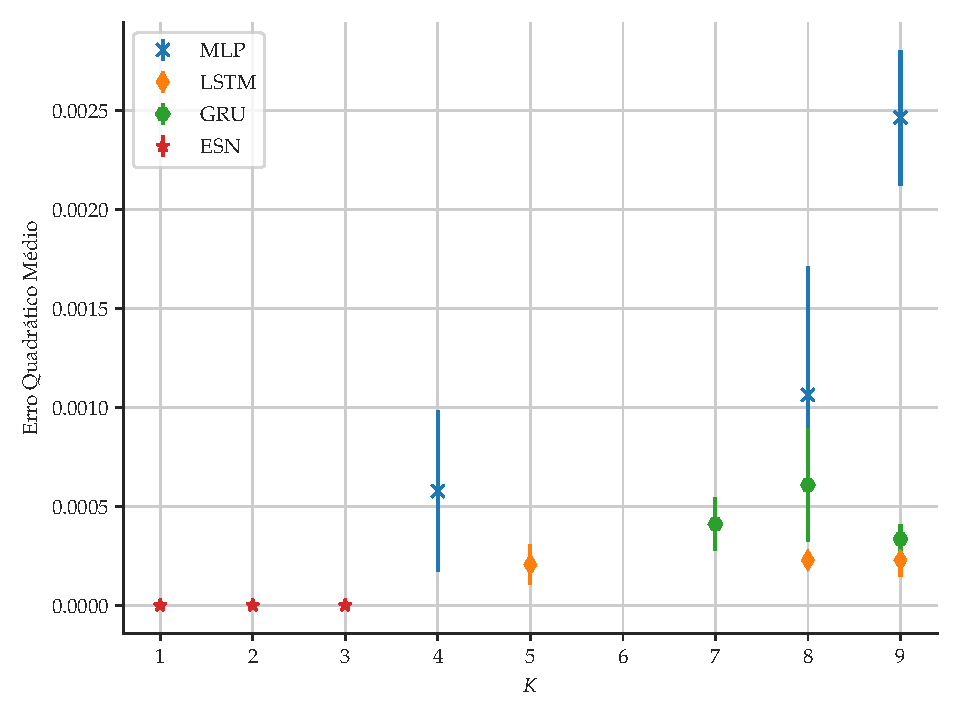
\includegraphics[scale=0.4]{henon-3best.pdf}
         \caption{Mapa de Hénon}
     \end{subfigure}
     \centering
     \begin{subfigure}[t]{0.45\textwidth} 
         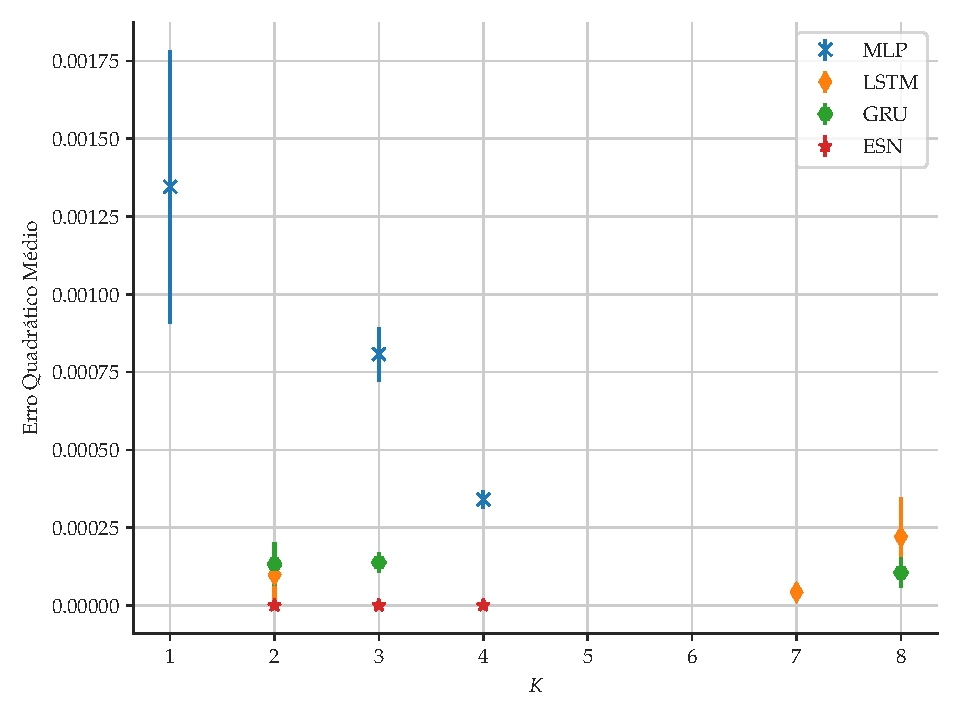
\includegraphics[scale=0.4]{logistic-3best.pdf}
         \caption{Mapa logístico}
     \end{subfigure}
     \\
     \centering
     \begin{subfigure}[t]{0.45\textwidth}
         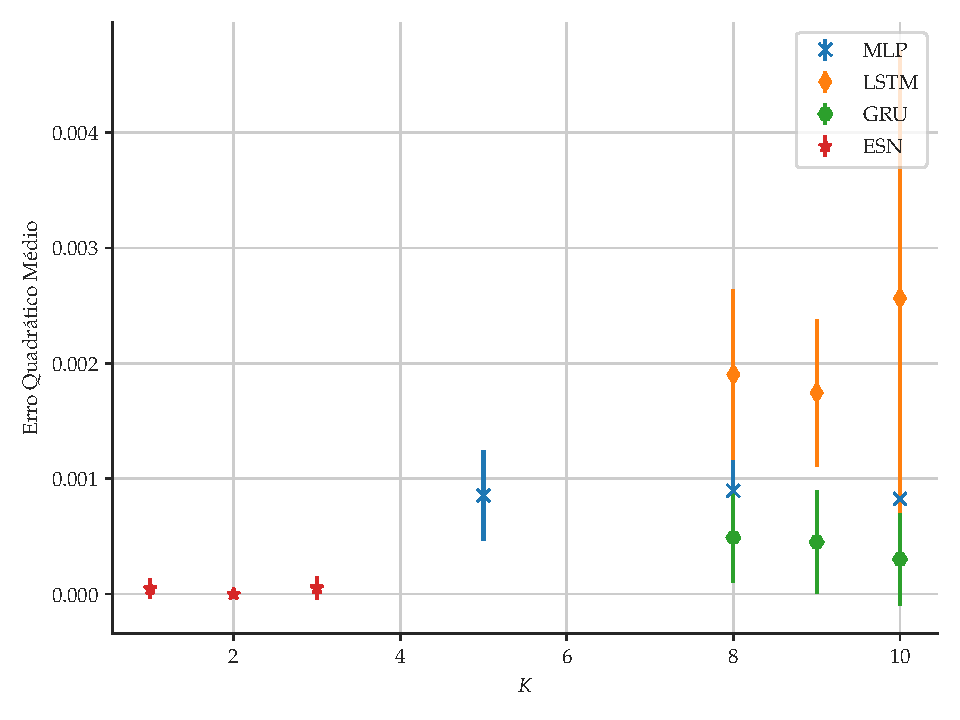
\includegraphics[scale=0.4]{lorenz-3best.pdf}
         \caption{Sistema de Lorenz}
     \end{subfigure}
     \centering
     \begin{subfigure}[t]{0.45\textwidth} 
         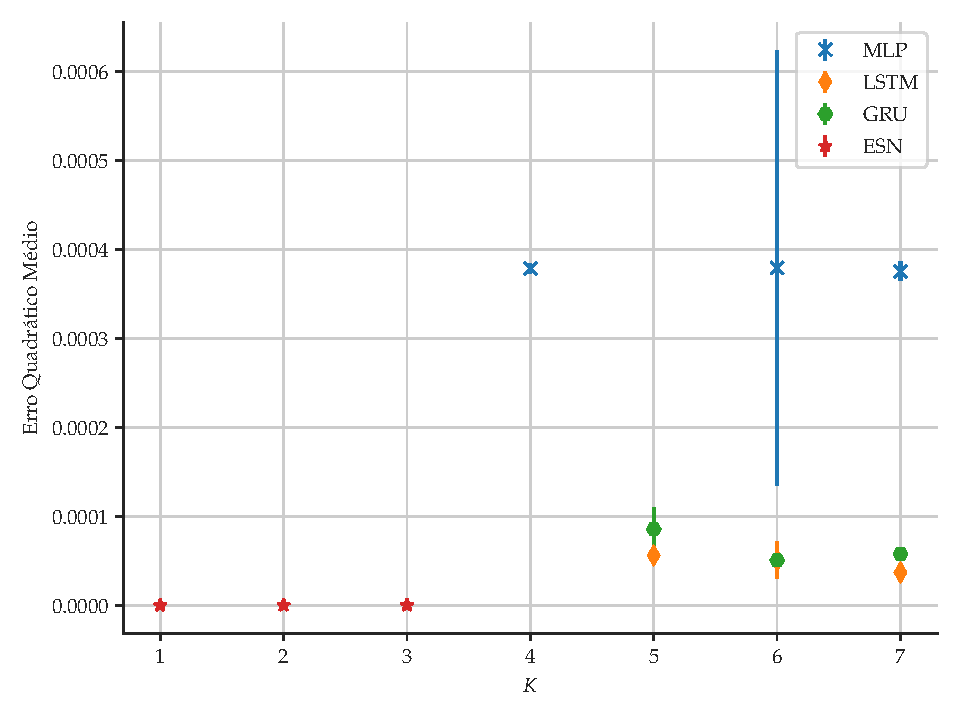
\includegraphics[scale=0.4]{mackeyglass-3best.pdf}
         \caption{Equações de Mackey-Glass}
     \end{subfigure}  
     \centering   
     \caption{Progressão do erro quadrático médio para os três melhores valores de $K$ nos cenários avaliados para todas as redes neurais testadas.}
     \label{fig:mse-progression-3best}
\end{figure}

\begin{table}[!ht]
\begin{center}
\begin{subtable}{0.35\textwidth}
\begin{center}
\scalebox{0.6}{
\begin{tabular}{c c c}
\toprule
\addlinespace
{\centering \textbf{Modelo}} & $\bm{K}$ & {\centering \textbf{Erro Quadrático Médio}}\\
   \addlinespace
 \midrule
 \addlinespace
 & 4 & $(5.780 \pm 4.047) \times 10^{-4}$\\
 \addlinespace
 {\centering \textbf{MLP}} & 8 & $(1.064 \pm 0.648) \times 10^{-3}$ \\
 \addlinespace
 & 9 & $(2.464 \pm 0.341) \times 10^{-3}$\\
 \addlinespace
 \hline
 \addlinespace
 & 8 & $(2.287 \pm 0.332) \times 10^{-4}$\\
 \addlinespace
 {\centering \textbf{LSTM}} & 9 & $(2.293 \pm 0.813) \times 10^{-4}$\\ 
 \addlinespace
 & 5 & $(2.063 \pm 0.994) \times 10^{-4}$\\
 \addlinespace
 \hline
 \addlinespace
 & 8 & $(6.083 \pm 2.839) \times 10^{-4}$\\
 \addlinespace
 {\centering \textbf{GRU}} & 9 & $(3.389 \pm 0.727) \times 10^{-4}$\\ 
 \addlinespace
 & 7 & $(4.104 \pm 1.354) \times 10^{-4}$\\
 \addlinespace
 \hline
 \addlinespace
  & 1 & $(3.251 \pm 0.536) \times 10^{-9}$\\
 \addlinespace
 {\centering \textbf{ESN}} & 2 & $(1.311 \pm 0.366) \times 10^{-8}$\\ 
 \addlinespace 
 & 3 & $(8.867 \pm 2.472) \times 10^{-8}$\\ 
 \bottomrule
\end{tabular}}
\caption{Mapa de Hénon}
\label{tab:henon-eqm-3best}
\end{center}
\end{subtable}
\begin{subtable}{0.35\textwidth}
\begin{center}
\scalebox{0.6}{
\begin{tabular}{c c c}
\toprule
\addlinespace
{\centering \textbf{Modelo}} & $\bm{K}$ & {\centering \textbf{Erro Quadrático Médio}}\\
   \addlinespace
 \midrule
 \addlinespace
 & 4 & $(3.403 \pm 0.292) \times 10^{-4}$\\
 \addlinespace
 {\centering \textbf{MLP}} & 3 & $(8.069 \pm 0.859) \times 10^{-4}$ \\
 \addlinespace
 & 1 & $(1.346 \pm 0.438) \times 10^{-3}$\\
 \addlinespace
 \hline
 \addlinespace
 & 2 & $(9.874 \pm 8.623) \times 10^{-5}$\\
 \addlinespace
 {\centering \textbf{LSTM}} & 7 & $(4.248 \pm 2.074) \times 10^{-5}$ \\ 
 \addlinespace
 & 8 & $(2.206 \pm 1.250) \times 10^{-4}$\\
 \addlinespace
 \hline
 \addlinespace
 & 8 & $(1.054 \pm 0.489) \times 10^{-4}$\\
 \addlinespace
 {\centering \textbf{GRU}} & 2 & $(1.320 \pm 0.687) \times 10^{-4}$\\ 
 \addlinespace
 & 3 & $(1.379 \pm 0.335) \times 10^{-4}$\\
 \addlinespace
 \hline
 \addlinespace
 & 2 & $(9.254 \pm 2.344) \times 10^{-9}$\\ 
 \addlinespace
 {\centering \textbf{ESN}} & 3 & $(1.157 \pm 0.500) \times 10^{-8}$\\ 
 \addlinespace 
 & 4 & $(6.064 \pm 1.851) \times 10^{-7}$\\ 
 \bottomrule
\end{tabular}}
\caption{Mapa logístico}
\label{tab:logistic-eqm-3best}
\end{center}
\end{subtable}
\begin{subtable}{0.35\textwidth}
\begin{center}
\scalebox{0.6}{
\begin{tabular}{c c c}
\addlinespace
\addlinespace
\addlinespace
\toprule
\addlinespace
{\centering \textbf{Modelo}} & $\bm{K}$ & {\centering \textbf{Erro Quadrático Médio}}\\
   \addlinespace
 \midrule
 \addlinespace
 & 5 & $(8.542 \pm 3.905) \times 10^{-4}$\\
 \addlinespace
 {\centering \textbf{MLP}} & 10 & $(8.266 \pm 5.422) \times 10^{-4}$ \\ 
 \addlinespace
 & 8 & $(8.945 \pm 4.267) \times 10^{-4}$\\
 \addlinespace
 \hline
 \addlinespace
 & 10 & $(2.564 \pm 2.149) \times 10^{-3}$\\
 \addlinespace
 {\centering \textbf{LSTM}} & 8 & $(1.903 \pm 0.738) \times 10^{-3}$\\ 
 \addlinespace
 & 9 & $(1.744 \pm 0.638) \times 10^{-4}$\\
 \addlinespace
 \hline
 \addlinespace
 & 10 & $(3.020 \pm 3.998) \times 10^{-4}$\\
 \addlinespace
 {\centering \textbf{GRU}} & 9 & $(4.512 \pm 4.481) \times 10^{-4}$\\ 
 \addlinespace
 & 8 & $(4.905 \pm 3.868) \times 10^{-4}$\\
 \addlinespace
 \hline
 \addlinespace
 & 2 & $(1.792 \pm 1.593) \times 10^{-6}$\\
 \addlinespace
 {\centering \textbf{ESN}} & 1 & $(4.833 \pm 8.416) \times 10^{-5}$\\ 
 \addlinespace 
 & 3 & $(5.384 \pm 9.854) \times 10^{-5}$\\
 \bottomrule
\end{tabular}}
\caption{Sistema de Lorenz}
\label{tab:lorenz-eqm-3best}
\end{center}
\end{subtable}
\begin{subtable}{0.35\textwidth}
\begin{center}
\scalebox{0.6}{
\begin{tabular}{c c c}
\addlinespace
\addlinespace
\addlinespace
\toprule
\addlinespace
{\centering \textbf{Modelo}} & $\bm{K}$ & {\centering \textbf{Erro Quadrático Médio}}\\
   \addlinespace
 \midrule
 \addlinespace
 & 4 & $(3.786 \pm 0.054) \times 10^{-4}$\\
 \addlinespace
 {\centering \textbf{MLP}} & 7 & $(3.756 \pm 0.105) \times 10^{-4}$ \\ 
 \addlinespace
 & 6 & $(3.795 \pm 2.441) \times 10^{-3}$\\
 \addlinespace
 \hline
 \addlinespace
 & 7 & $(3.750 \pm 1.016) \times 10^{-5}$\\
 \addlinespace
 {\centering \textbf{LSTM}} & 6 & $(5.089 \pm 2.077) \times 10^{-5}$\\ 
 \addlinespace
 & 5 & $(5.638 \pm 0.208) \times 10^{-5}$\\
 \addlinespace
 \hline
 \addlinespace
 & 7 & $(5.817 \pm 0.633) \times 10^{-5}$\\
 \addlinespace
 {\centering \textbf{GRU}} & 5 & $(8.594 \pm 2.413) \times 10^{-5}$\\  
 \addlinespace
 & 6 & $(5.101 \pm 0.938) \times 10^{-5}$\\
 \addlinespace
 \hline
 \addlinespace
 & 1 & $(4.812 \pm 0.378) \times 10^{-7}$\\
 \addlinespace
 {\centering \textbf{ESN}} & 2 & $(6.493 \pm 0.572) \times 10^{-7}$\\  
 \addlinespace
 & 3 & $(7.789 \pm 0.221) \times 10^{-7}$\\ 
 \bottomrule
\end{tabular}}
\caption{Equações de Mackey-Glass}
\label{tab:mackeyglass-eqm-3best}
\end{center}
\end{subtable}
\caption{Valores médios e desvios-padrão do erro quadrático médio obtidos para cada $K$ nos cenários utilizadas.}
\label{tab:eqm-results-3best}
\end{center}
\end{table}

Finalmente, depois de visualizarmos a progressão do EQM nos três melhores valores de $K$ para cada caso, selecionamos os melhores para o último teste realizado, novamente, seguindo o procedimento descrito no início desta seção.

A próxima seção exibe os resultados obtidos, juntamente com certos trechos das predições onde a diferença entre os modelos foi perceptível.

\section{Resultados}

Após identificarmos o melhor valor de $K$ para cada modelo, realizou-se novamente o processo mencionado na seção anterior e foi obtido o EQM de teste para as melhores configurações (parâmetros e $K$) para cada modelo, em todos os cenários. 

A figura \ref{fig:model-comparison} exibe o comparativo dos melhores desempenhos das redes neurais analisadas, e a figura \ref{fig:series-comparison} mostra uma comparação da predição em si de cada modelo em certos trechos das séries temporais nos quais a diferença foi mais perceptível visualmente.
\begin{figure}[H]
     \begin{subfigure}[t]{0.45\textwidth}
         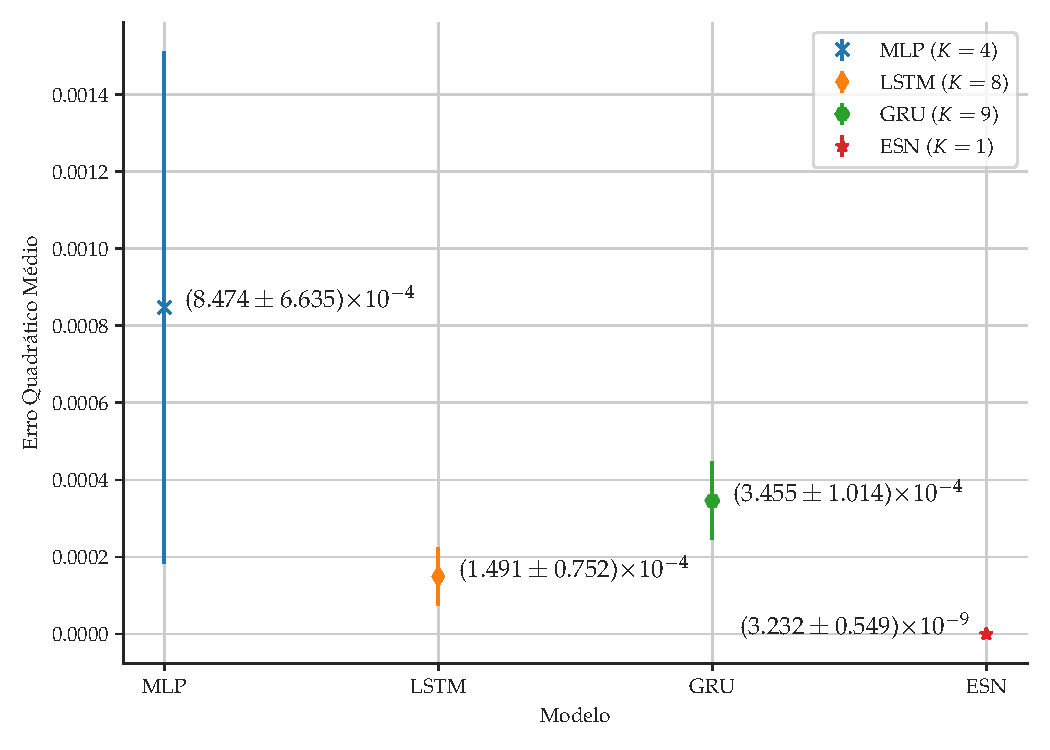
\includegraphics[scale=0.385]{comparacao-k-henon.pdf}
         \caption{Mapa de Hénon}
     \end{subfigure}
     \centering
     \begin{subfigure}[t]{0.45\textwidth} 
         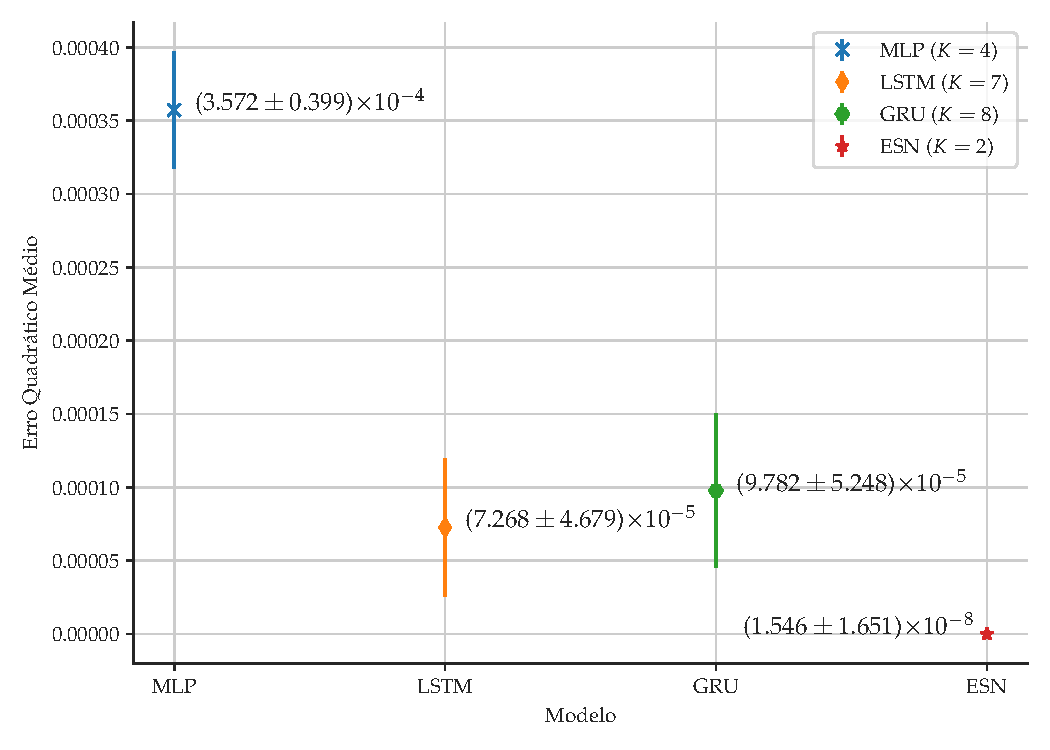
\includegraphics[scale=0.385]{comparacao-k-logistic.pdf}
         \caption{Mapa logístico}
     \end{subfigure}
     \centering
     \\
     \begin{subfigure}[t]{0.45\textwidth}
         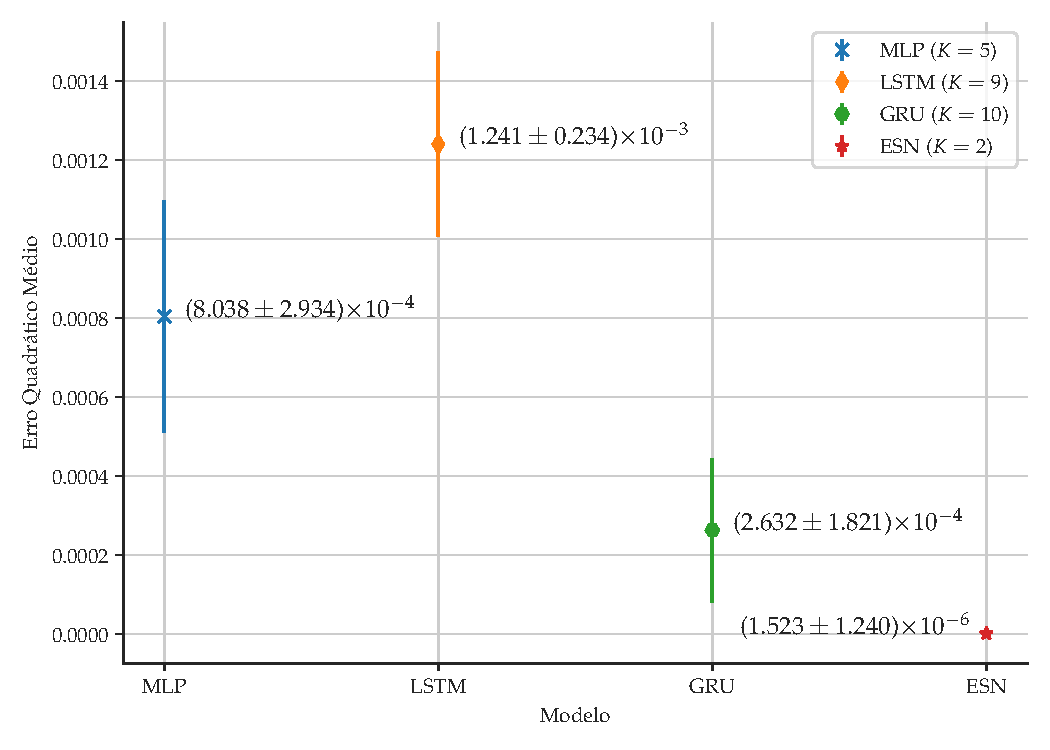
\includegraphics[scale=0.385]{comparacao-k-lorenz.pdf}
         \caption{Sistema de Lorenz}
     \end{subfigure}
     \centering
     \begin{subfigure}[t]{0.45\textwidth} 
         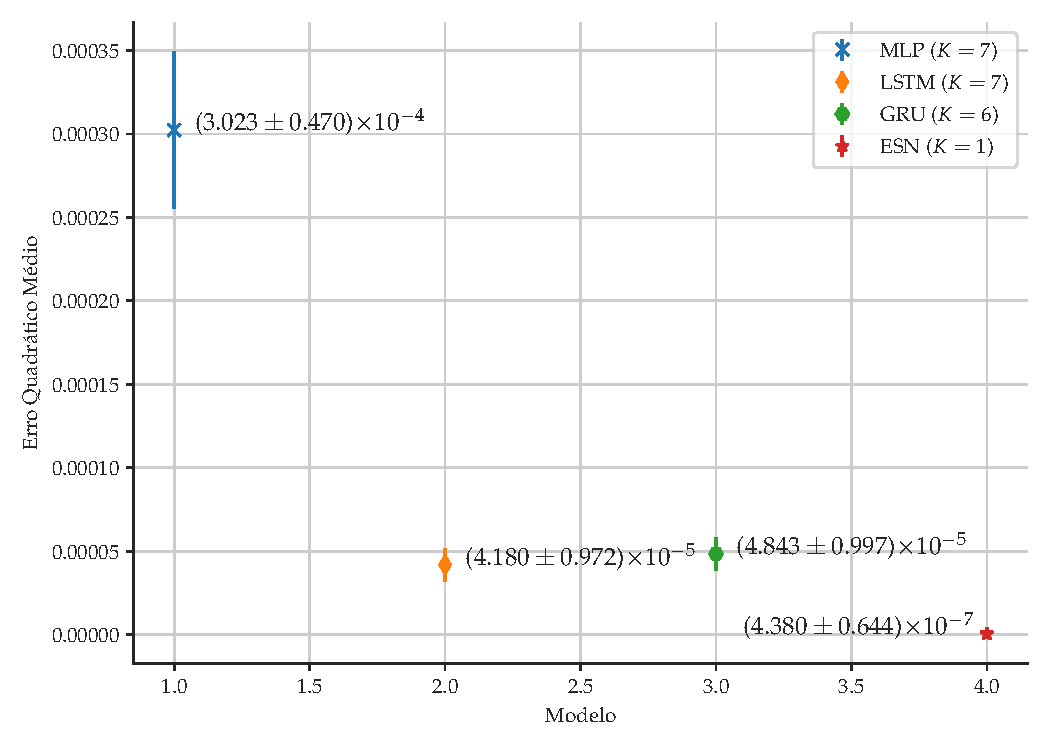
\includegraphics[scale=0.385]{comparacao-k-mackeyglass.pdf}
         \caption{Equações de Mackey-Glass}
     \end{subfigure}  
     \centering   
     \caption{Comparação do melhor desempenho obtido por cada modelo nos cenários testados.}
     \label{fig:model-comparison}
\end{figure}
\begin{figure}[H]
     \begin{subfigure}[t]{0.4\textwidth} 
         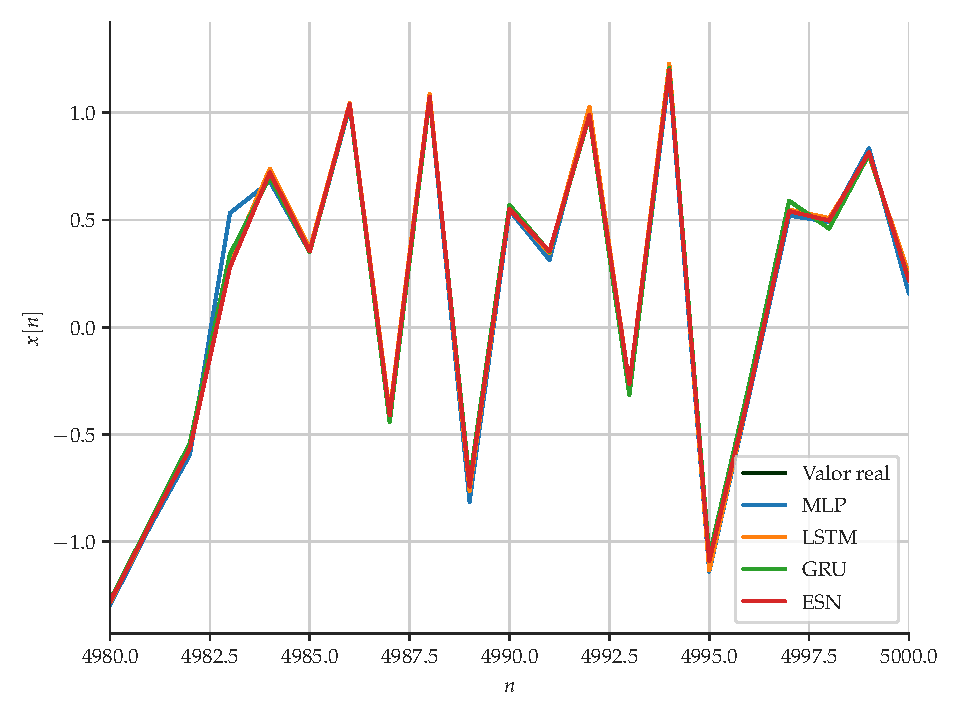
\includegraphics[scale=0.35]{vs-henon-zoom.pdf}
         \caption{Mapa de Hénon}
     \end{subfigure}
     \centering
     \begin{subfigure}[t]{0.4\textwidth} 
         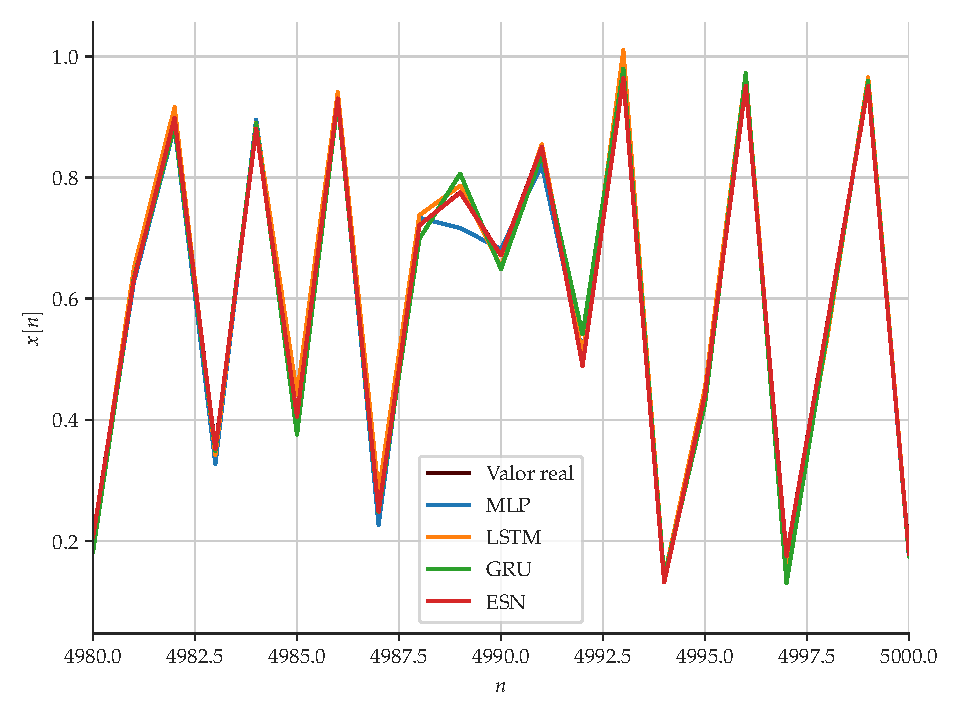
\includegraphics[scale=0.35]{vs-logistic-zoom.pdf}
         \caption{Mapa logístico}
     \end{subfigure}
     \centering
     \\
     \begin{subfigure}[t]{0.4\textwidth} 
         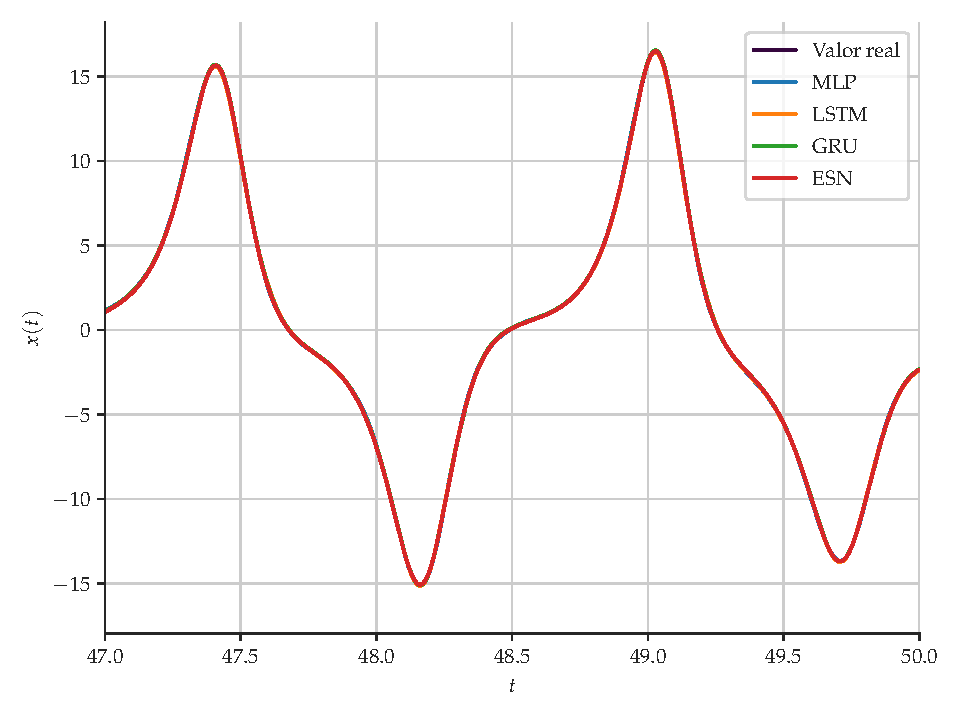
\includegraphics[scale=0.35]{vs-lorenz-zoom.pdf}
         \caption{Sistema de Lorenz}
     \end{subfigure}
     \centering
     \begin{subfigure}[t]{0.4\textwidth}
         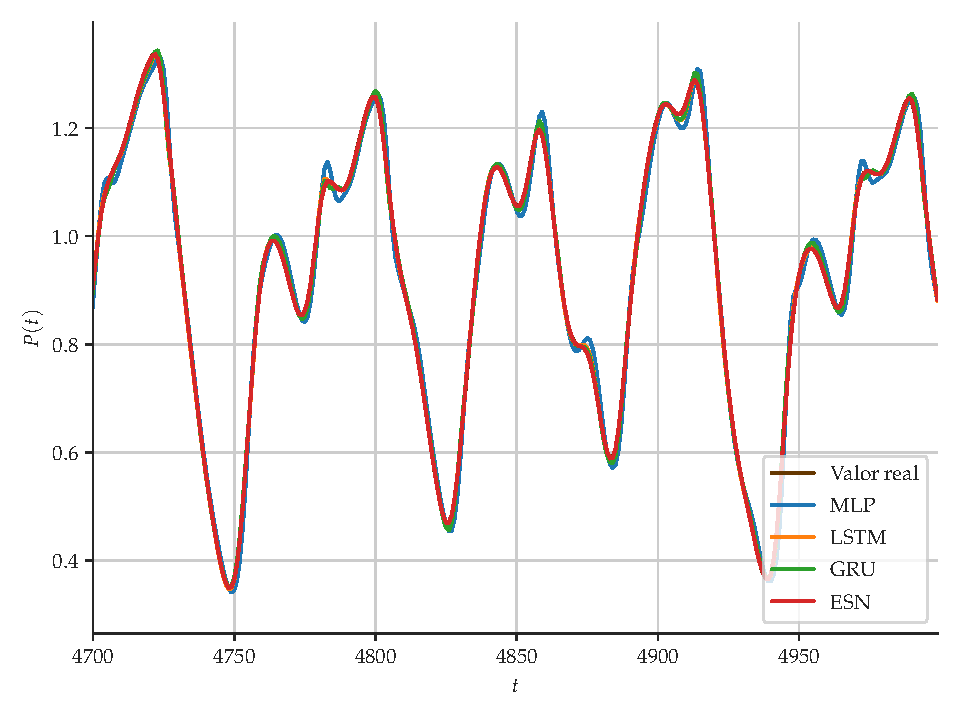
\includegraphics[scale=0.35]{vs-mackeyglass-zoom.pdf}
         \caption{Equações de Mackey-Glass}
     \end{subfigure}
     \centering     
     \caption{Comparação da predição realizada por cada modelo para os quatro sistemas caóticos.}
     \label{fig:series-comparison}
\end{figure}


\section{Análise e Conclusão}

Analisando os resultados obtidos, percebe-se que, com exceção do cenário do sistema de Lorenz, a rede MLP foi consideravelmente pior do que as redes recorrentes. Também percebe-se que, dentre as redes recorrentes, a ESN obteve um EQM bem inferior ao obtido pela LSTM e pela GRU.

O desempenho inferior da rede MLP com relação às redes recorrentes provavelmente decorre do fato de que a relação temporal presente na LSTM, GRU e ESN auxilia na modelagem da dinâmica da série temporal. Já o pior desempenho da LSTM na série temporal do sistema de Lorenz provavelmente está relacionado aos efeitos estocásticos presentes no ajuste dos pesos sinápticos dessa rede neural que, conforme indicado em \cite{doya1992bifurcations}, é uma dificuldade em seu treinamento.

Algo interessante de mencionar é que, no geral, os desempenhos de todos os modelos estudados foram consideravelmente bons nas séries temporais dos sistemas a tempo contínuo (sistema de Lorenz e equações de Mackey-Glass), sendo que as diferenças foram mais pronunciadas na série temporal do mapa de Hénon e do mapa logístico. Provavelmente, a maior suavidade presente nas séries de Lorenz e de Mackey-Glass facilita a modelagem do preditor, além do fato de que as séries temporais mencionadas são bem menos erráticas se comparadas às séries de Hénon e do mapa logístico.

O principal resultado observado foi que o modelo preditor utilizando a rede com estados de eco obteve um desempenho bem superior aos outros modelos, em todos os cenários. O erro quadrático médio foi tão baixo que, observando a predição nos dados de teste, praticamente não há diferença entre os valores reais e os valores previstos. Essa superioridade da ESN também é realçada na imagem  comparativa do EQM, que indica que a ESN  atingiu patamares de erro cerca de $100$ ou até $10000$ vezes menores que os outros modelos. 

Esse resultado, aliado ao fato de que o treinamento da ESN é bem menos custoso computacionalmente se comparado ao das outras redes, mostra que esta rede é uma boa alternativa para futuros estudos de modelos preditores de séries temporais. Além disso, conforme mostrado em outros trabalhos como \cite{jaeger2004harnessing, jaeger2007echo, boccato2013novas}, a ESN também é uma boa ferramenta para outras tarefas de extração de informação, como em equalização de canais e separação de fontes. 

Como sugestão de trabalhos futuros, pode ser avaliada a eficácia da ESN em reconstruir atratores através de séries temporais experimentais de sistemas caóticos. Se o desempenho para essa tarefa for tão bom quanto o obtido na predição das séries estudadas, a ESN pode tornar-se uma ferramenta ainda mais poderosa para a modelagem de sistemas com dinâmica caótica.

Com isso, finalizamos esta pesquisa de iniciação científica. Através dos processos descritos neste relatório final e, anteriormente, no relatório parcial, o aluno teve contato com ferramentas modernas de predição de séries temporais, úteis não só para séries originadas por dinâmicas caóticas, como também para cenários relacionados a outros tipos de sistemas.

Além disso, o aluno teve uma exposição a outras ferramentas de aprendizado de máquina que não necessariamente estão relacionadas com problemas de predição, mas que podem ser úteis para outros tipos de projetos de pesquisa que o estudante possa participar no futuro.

Logo, esse projeto forneceu os princípios para que o aluno possa atuar junto a diversas áreas do conhecimento, como a matemática, a física e até mesmo a biologia, e desenvolver pesquisas científicas bem fundamentadas, cumprindo, assim, o principal objetivo de um projeto de iniciação científica.


\bibliographystyle{ieeetr}

{\bibliography{bib}}

\pdfinfo{
   /Title  (Relatório EE016 - João Pedro O. Pagnan)
}

\end{document}